% This is "sig-alternate.tex" V2.0 May 2012
% This file should be compiled with V2.5 of "sig-alternate.cls" May 2012
%
% This example file demonstrates the use of the 'sig-alternate.cls'
% V2.5 LaTeX2e document class file. It is for those submitting
% articles to ACM Conference Proceedings WHO DO NOT WISH TO
% STRICTLY ADHERE TO THE SIGS (PUBS-BOARD-ENDORSED) STYLE.
% The 'sig-alternate.cls' file will produce a similar-looking,
% albeit, 'tighter' paper resulting in, invariably, fewer pages.
%
% ----------------------------------------------------------------------------------------------------------------
% This .tex file (and associated .cls V2.5) produces:
%       1) The Permission Statement
%       2) The Conference (location) Info information
%       3) The Copyright Line with ACM data
%       4) NO page numbers
%
% as against the acm_proc_article-sp.cls file which
% DOES NOT produce 1) thru' 3) above.
%
% Using 'sig-alternate.cls' you have control, however, from within
% the source .tex file, over both the CopyrightYear
% (defaulted to 200X) and the ACM Copyright Data
% (defaulted to X-XXXXX-XX-X/XX/XX).
% e.g.
% \CopyrightYear{2007} will cause 2007 to appear in the copyright line.
% \crdata{0-12345-67-8/90/12} will cause 0-12345-67-8/90/12 to appear in the copyright line.
%
% ---------------------------------------------------------------------------------------------------------------
% This .tex source is an example which *does* use
% the .bib file (from which the .bbl file % is produced).
% REMEMBER HOWEVER: After having produced the .bbl file,
% and prior to final submission, you *NEED* to 'insert'
% your .bbl file into your source .tex file so as to provide
% ONE 'self-contained' source file.
%
% ================= IF YOU HAVE QUESTIONS =======================
% Questions regarding the SIGS styles, SIGS policies and
% procedures, Conferences etc. should be sent to
% Adrienne Griscti (griscti@acm.org)
%
% Technical questions _only_ to
% Gerald Murray (murray@hq.acm.org)
% ===============================================================
%
% For tracking purposes - this is V2.0 - May 2012

\documentclass{sig-alternte-cosn}

\usepackage{times}
\usepackage{helvet}
\usepackage{courier}

\usepackage{amsmath,amsfonts,amssymb}%,amsthm}
\usepackage{array}
\usepackage{amsmath,amssymb}
\usepackage[lofdepth,lotdepth]{subfig}
\usepackage{graphicx}
\usepackage{epstopdf}
\usepackage{color}
\usepackage[pdftex]{hyperref}

%\usepackage{hyperref}
\frenchspacing

\newcommand{\link}{\mathit{link}}
\newcommand{\post}{\mathit{post}}
\newcommand{\photo}{\mathit{photo}}
\newcommand{\video}{\mathit{video}}
\newcommand{\ttag}{\mathit{tag}}
\newcommand{\comment}{\mathit{comment}}
\newcommand{\incoming}{\mathit{incoming}}
\newcommand{\outgoing}{\mathit{outgoing}}
\newcommand{\all}{\mathit{all}}
\newcommand{\app}{\mathit{app}}

% place holder spacing hacks
\newcommand{\secmoveup}{\vspace{-1.2mm}}                %{\vspace{-0.12in}}
\newcommand{\bigsecmoveup}{\secmoveup\vspace{-.0mm}}   %{\vspace{-0.08in}}

\newcommand{\textmoveup}{\vspace{-0mm}}               %{\vspace{-0.08in}}
\newcommand{\bigtextmoveup}{\textmoveup\vspace{-0.0in}} %{\vspace{-0.06in}}
\newcommand{\itemmoveup}{\vspace{-0mm}}              %{\vspace{-0.04in}}
\newcommand{\eqmoveup}{\vspace{-0.0in}}                 %{\vspace{-0.16in}}
\newcommand{\captionmoveup}{\eqmoveup\vspace{-0.0in}}   %{\vspace{-0.16in}}
\newcommand{\refitemmoveup}{\vspace{-0mm}}            %{\vspace{-0.16in}}
% hold but hide chunks of text
\newcommand{\eat}[1]{}
\newcommand{\yum}{}
\newcommand{\TODO}[1]{ {\color{blue}{\bf TODO:~{#1}}} }
\newcommand{\surl}[1]{\urlstyle{same}\url{#1}}

%\newcommand{}{\mathit{}}
\newcommand{\x}{\mathbf{X}}
\newcommand{\otherwise}{\mathit{otherwise}}
\newcommand{\unknown}{\mathit{unknown}}
\newcommand{\dislike}{\mathit{dislike}}
\newcommand{\like}{\mathit{likes}}
\newcommand{\likes}{\mathit{likes}}
\newcommand{\true}{\mathit{true}}
\newcommand{\false}{\mathit{false}}
\def\argmax{\operatornamewithlimits{arg\,max}}
\def\argmin{\operatornamewithlimits{arg\,min}}

\begin{document}
%
% --- Author Metadata here ---
\conferenceinfo{COSN}{'13 BOSTON, USA}
%\CopyrightYear{2007} % Allows default copyright year (20XX) to be over-ridden - IF NEED BE.
%\crdata{0-12345-67-8/90/01}  % Allows default copyright data (0-89791-88-6/97/05) to be over-ridden - IF NEED BE.
% --- End of Author Metadata ---

\title{Social Affinity Filtering: Recommendation through \\Fine-grained Analysis of User Interactions and Activities}

\numberofauthors{6} %  in this sample file, there are a *total*
% of EIGHT authors. SIX appear on the 'first-page' (for formatting
% reasons) and the remaining two appear in the \additionalauthors section.
%


% You can go ahead and credit any number of authors here,
% e.g. one 'row of three' or two rows (consisting of one row of three
% and a second row of one, two or three).
%
% The command \alignauthor (no curly braces needed) should
% precede each author name, affiliation/snail-mail address and
% e-mail address. Additionally, tag each line of
% affiliation/address with \affaddr, and tag the
% e-mail address with \email.
%
% 1st. author
\author{
\alignauthor
% 1st
Suvash Sedhain\\
       \affaddr{ANU \& NICTA}\\
       \affaddr{Canberra, Australia}\\
	   \email{ssedhain@nicta.com.au}
% 2nd. author
	\alignauthor Scott Sanner\\
       \affaddr{NICTA \& ANU}\\
       \affaddr{Canberra, Australia}\\
       \email{ssanner@nicta.com.au}
% 3rd. author
\alignauthor Lexing Xie\\
       \affaddr{ANU \& NICTA}\\
       \affaddr{Canberra, Australia}\\
       \email{lexing.xie@anu.edu.au}
\and  % use '\and' if you need 'another row' of author names
% 4th. author
\alignauthor Riley Kidd\\
	\affaddr{ANU}\\
	\affaddr{Canberra, Australia}\\
	\email{rileyjkidd@gmail.com}
% 5th. author
\alignauthor Khoi-Nguyen Tran\\
	\affaddr{ANU}\\
	\affaddr{Canberra, Australia}\\
	\email{kndtran@cs.anu.edu.au}
% 6th. author	
\alignauthor Peter Christen\\
	\affaddr{ANU}\\
	\affaddr{Canberra, Australia}\\
	\email{peter.christen@anu.edu.au}
}

% There's nothing stopping you putting the seventh, eighth, etc.
% author on the opening page (as the 'third row') but we ask,
% for aesthetic reasons that you place these 'additional authors'
% in the \additional authors block, viz.

%\additionalauthors{Additional authors: John Smith (The Th{\o}rv{\"a}ld Group,
%email: {\texttt{jsmith@affiliation.org}}) and Julius P.~Kumquat
%(The Kumquat Consortium, email: {\texttt{jpkumquat@consortium.net}}).}

%\date{30 July 1999}

% Just remember to make sure that the TOTAL number of authors
% is the number that will appear on the first page PLUS the
% number that will appear in the \additionalauthors section.

\maketitle
\begin{abstract}
Content recommendation in social networks poses the complex problem of
learning user preferences from a rich and complex set of interactions
(e.g., likes, comments and tags for posts, photos and videos) and
activities (e.g., favourites, group memberships, page likes).  While
many social collaborative filtering approaches learn from aggregate statistics over this
social information, we propose a different approach: we first define
social affinity groups (SAGs) of a target user by analysing their
fine-grained interactions (e.g., users who have been tagged in the
target user's video) and activities (e.g., users who have joined the
same interest group that the target user has joined).  Then we
learn which SAGs are most predictive of the target user's preferences
in a method we term social affinity filtering (SAF).  We apply SAF to
preference data from a set of Facebook users and their
complete interactions with 38,000+ friends collected over a four month
period.  Our analysis demonstrates that SAF yields higher accuracy
than a range of state-of-the-art (social) collaborative filtering approaches and that not all
interactions and activities are equally predictive: among many insights, 
we show certain user-to-user interactions are more
informative than others %(tagging is often more informative than
%commenting, video interactions are more informative than wall post
%interactions)
%we analyse trends in the relationship between the
%size of activity-based SAGs and informativeness
% (small groups can be
%highly informative while large groups are rarely informative).
and we show that activity informativeness varies drastically with type and size.
 In summary, this work demonstrates the previously untapped
predictive power of fine-grained social interaction and activity
features and the novel method of SAF to leverage them for
state-of-the-art social recommender systems.


\end{abstract}

% A category with the (minimum) three required fields
\category{H.3.3}{Information Search and Retrieval}{Information Filtering}
%A category including the fourth, optional field follows...
%\category{D.2.8}{Software Engineering}{Metrics}[complexity measures, performance measures]

%\terms{Theory}

\keywords{social networks, collaborative filtering, recommender systems}

\section{Introduction}

%!TEX root = document.tex

\label{sec:introduction}

% motivate socical recommendation 
Online social networks such as Facebook record a rich set of user
preferences (likes of links, posts, photos, videos), user traits,
interactions and activities (conversation streams, tagging, group
memberships, interests, personal history and demographic data).  
This presents myriad new
dimensions to the recommendation problem by making available a rich
labeled graph structure of social content from which user preferences
can be learned and new recommendations can be made.  

Existing recommendation methods for social networks aggregate this
rich social information into a simple measure of user-to-user interaction 
that can be leveraged to model user homophily via social
regularization~\cite{lla,socinf,sr,rrmf, Noel2012NOF}, a trust
ensemble~\cite{ste}, or a low-rank factorization of the social
interactions matrix~\cite{sorec}.  But in aggregating all of these
interactions and common activities into a single strength of
interaction, we ask whether important preference information has been
discarded?  Indeed, the point of departure for this work is the
hypothesis that different fine-grained interactions (e.g. commenting
on a wall vs. getting tagged in a video) and activities (e.g., a
university alumni group vs fans of a TV series) \emph{do} represent different
preferential {\em affinities} between users, and moreover that effective
{\em filtering} of this information will lead to better results in
social recommendation.

%% No longer fits cleanly in the intro, should be moved into related
%% work is not already mentioned there.  -SPS
\eat{
In the context of recent work on social
recommendation~\cite{sorec,ste,lla} and information diffusion
~\cite{Goel2012structure,Romero2011hashtag,Bakshy2012chamber}, it is
important to know which of these interactions or common traits are
actually reflective of common preferences.}

To quantitatively validate our hypotheses and evaluate the
informativeness of different fine-grained features for social
recommendation, we have built a Facebook App to collect detailed user
interaction and activity history available through the Facebook Graph
API along with preferences solicited from the App regarding recommendations.
Specifically, our App recommends three daily links to each
App user collected from the timeline of other users (both friends and
non-friends) and we record users' explicit likes and dislikes of these
recommended links.  Given this data, we define \emph{social affinity
groups (SAGs)} of a target user by analysing their fine-grained
interactions (e.g., users who have been tagged in the target user's
video) and activities (e.g., users who have joined the same special
interest group that the target user has joined).  Given these SAGS, we
(a) learn to predict whether a user will like an item based on members
of other SAGs who have also liked the item using a novel
recommendation method we call {\em social affinity filtering (SAF)},
and (2) analyse the relative informativeness of different SAGs based
on various properties that we elaborate on next.

In our 4-month interaction trace, we were able to collect data for a set of 
Facebook app users and their full interactions with 38,000+ friends along with 22
distinct types of interaction and users activity for 3000+ groups, 4000+ favourites, and 10,000+ pages. 
In subsequent sections that outline our experimental methodology and results in detail, 
we have made the following important observations:
\begin{itemize}
\item We found that SAF significantly 
outperforms numerous state-of-the-art collaborative filtering and social recommender 
systems, by up to 6\% in accuracy -- in short, fine-grained 
interactions are extremely informative, bringing into question the efficacy of 
previous social recommendation approaches that aggregate user-to-user interactions into 
a single value.
% Also, what about combining all features?  Not enough data?  -SPS
% Probably also much faster -- should we show a table of train and test times?  -SPS
\item We also found that groups, pages, and favourites make for more informative
SAGs than those defined by user-to-user interactions -- likely because the former can be
applied to SAGs over the entire Facebook population 
rather than just a user's friends (where the data is considerably limited).
\item Among the interactions, we found that those on videos are more predictive than those on other content types (photos, post, link), and that outgoing interactions (performed by the ego) 
are more predictive than incoming ones (performed by friends on the ego's timeline).
% Below: not sure I quite understand ``persistent'' and ``temporally synchronized'' here... 
% are there better terms or can they be further (briefly) explained?
\item Among {\em groups}, {\em pages} and {\em favourites}, we found that the most  
predictive features have smaller membership size, and that favourite features corresponding to 
persistent activities (such as TV, books, activities) are more predictive than generic or 
temporally synchronized activities (such as interests, sports). 
\end{itemize}
As detailed in the subsequent sections, these findings 
not only demonstrate the power of leveraging fine-grained
interaction and activity features but they also suggest which features are most
important to collect when building SAF-based recommenders.


\eat{
To better understand these subtleties and to understand what
social interactions and user traits reflect common preferences on
Facebook, we proceed in the following sections to describe our data,
our experimental methodology, and various analyses according to our
methodology that shed light on the above questions. 
On one hand our observations confirm certain observations made previous 
on different networks, such as the diminishing returns of repeated exposures, 
on the other we also see a few new clues such as 
that very specific types of outgoing interactions are more predictive 
than other interactions. 
We then conclude with a summary of the key novel observations arising
from this study.
}

\yum



\section{Social Affinity Filtering}
\label{sec:methodology}
%!TEX root = document.tex

\begin{figure}[t!]
\centering
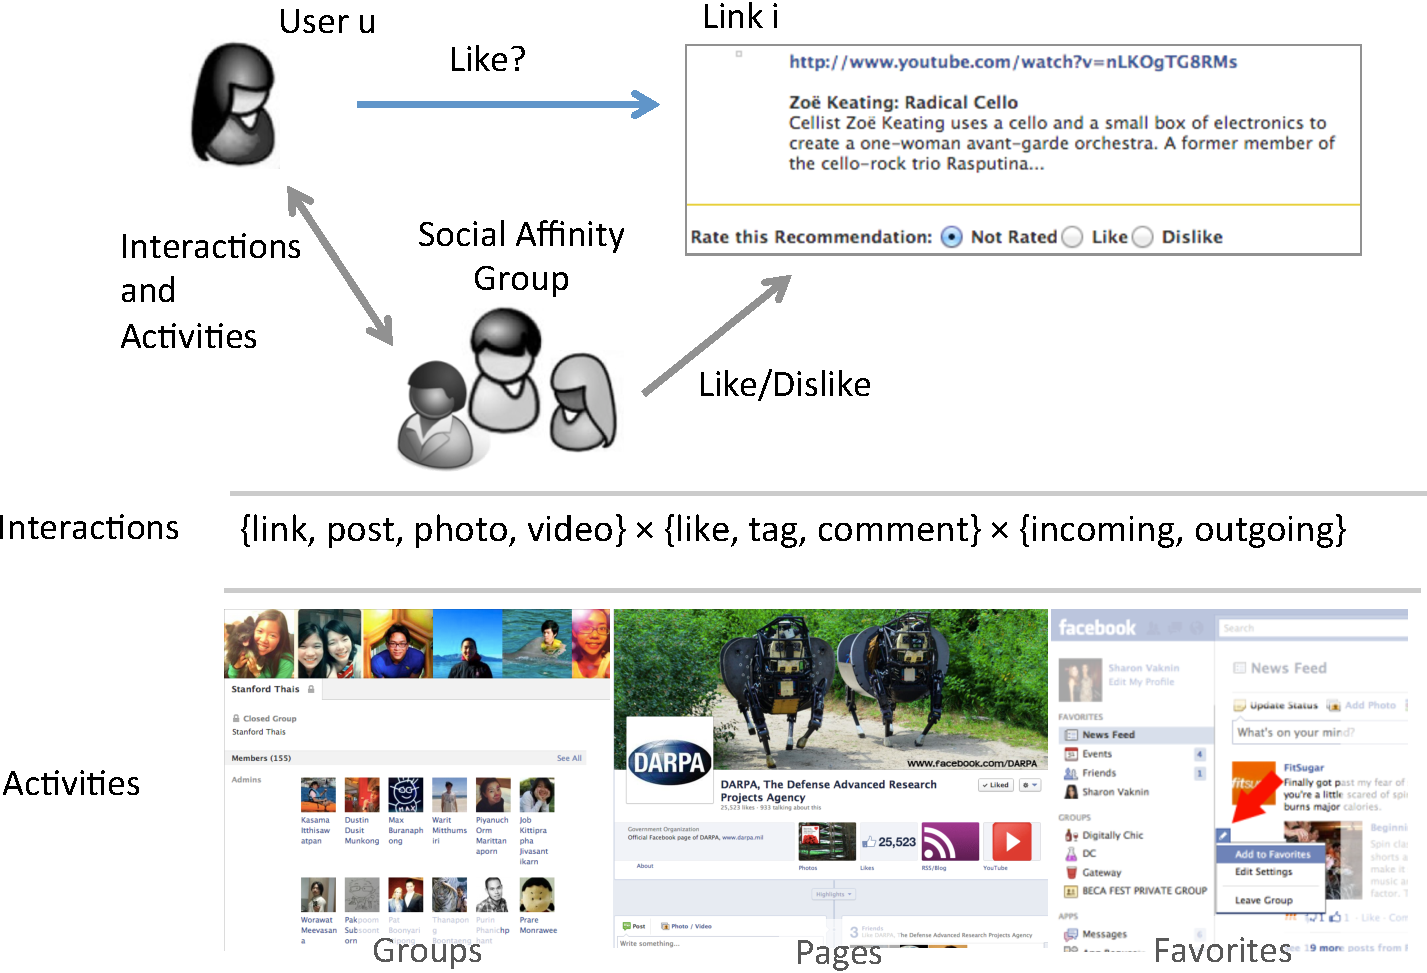
\includegraphics[width=.95\linewidth]{data/overview}
\caption{Overview of social affinity for link recommendation.}
\label{fig:overview}
\end{figure}


As illustrated in Fig~\ref{fig:overview}, the high-level objective of this paper is to predict whether or not a user $u$ will like a digital item $i$ (in our test case, a link). 
We define user $u$'s preference for link $i$ as $like(u,i)$, this will be our prediction target. 
\begin{quote}
\begin{math}
likes(u,i) =  \begin{Bmatrix}
	  True & \text{if user $u$ likes item $i$}\\
	  False & \text{otherwise}
	  \end{Bmatrix}
\end{math}
\end{quote}

We define the social affinity between two users via their direct {\em interactions}
on various digital items, and their shared {\em activities} in different communities of the social network. 
We call our recommendation algorithm \textit{Social Affinity Filtering (SAF)}, as it infers 
$like(u,i)$ through the preference of their 
\textit{ Social Affinity Groups (SAG)}, i.e. a set of users with known preferences to link $i$, and who has at least one interaction or activity in common with $u$. 

\subsection{Action types on Facebook}
On Facebook, We use the term {\em Interactions} and {\em Activities} to refer to the range of user-user and user-community actions, respectively.

\noindent {\bf Interactions} describes the communication between Facebook users. There are a few dozen different interaction types that have distinct item modality, action and direction.
\begin{itemize}
\item \textbf{Modality:} (4 possibilities)
User $u$ can interact with another user $v$ via \textit{links, posts, photos} and \textit{videos} that appear in either user's timeline.

\item \textbf{Action type:} (3 possibilities)
A user $u$ can \textit{comment} or \textit{like} 
user $v$'s item. He/she can also \textit{tag} user $v$ on an 
item, often indicating that user $v$ is present when the content is created (for photo/video/post), 
or to explicitly raise user $v$'s attention for a post -- with one exception in Facebook that $u$ cannot tag a link with users $v$ since the link is created by third parties and merely shared on Facebook.

\item \textbf{Directionality:} (2 possibilities)
We look at \textit{incoming} and \textit{outgoing} interactions, i.e.,
if user $u$ comments on, tags, or likes user $v$'s item,
then this is an outgoing interactions for $u$, and an incoming interactions for $v$.
Although high correlation between \textit{incoming} and \textit{outgoing} interactions 
is recently observed~\cite{saez2011high}, whether or not interaction direction 
affects user preferences differently is still an open question we wish to answer
in this work. 
%then $u$ is in the set of incoming interactions for $v$
%and $v$ is in the set of outgoing interactions for $u$.
      								
\end{itemize}
There are a total of 22 interaction types. Namely the cross-product of modalities, actions and directions, minus {\em link-tag-\{incoming, outgoing\}}. 

%\subsection{Activities}
\noindent{\bf Activities} describes the user interactions with Facebook communities like groups, pages, favourites.
\begin{itemize}
  %@SCOTT/LEXING following defination are taken from facebook blog. I am confused how to cite it %
  \item \textbf{Groups} on Facebook 
\footnote{According to Facebook Blog (\surl{https://www.facebook.com/blog}), ``Groups are the place for small group communication and for people to share their common interests and express their opinion. Groups allow people to come together around a common cause, issue or activity to organize, express objectives, discuss issues, post photos and share related content''. 
\label{fn:fbblog}}
are analogous to community organizations in the real-world. It allows users to declare membership and supports people to organize activities, to post related content, and to have recurring discussions about them.  Examples of groups include {\em Stanford Thai} (Fig~\ref{fig:overview} bottom left), or {\em Harvard Debate Club}.
  \item \textbf{Pages} on Facebook
  \footnote{According to Facebook Blog, ``Facebook Pages enable public figures, businesses, organizations and other entities to create an authentic and public presence on Facebook. Facebook Pages are visible to everyone on the internet by default. Facebook user can connect with these Pages by becoming a fan and then receive their updates and interact with them.'' }
  %\footnotemark[\ref{fn:fbblog}] 
  are analogous to the homepages of people, organizations and events on the world-wide-web. They are publicly visible, and users can subscribe to the updates on the page, and also engage in discussions. Example pages include {\em DARPA} (an organization, Fig~\ref{fig:overview} bottom middle), or {\em Beyonce} (a singer).

  \item \textbf{Favourites} are analogous to bookmarks (on physical books or on the web browser). It it is a user-created list containing various digital items such as Facebook apps, books, music, and many other types of items to indicate their interest. Example favourite items include {\em Big Bang Theory} (TV series), or {\em FC Barcelona} (soccer club). Fig~\ref{fig:overview} bottom right show a Facebook screenshot when a user adds a favourite.
  \footnote{According to Facebook Blog, ``Facebook facilitates a wide variety of user selected favourites (Activities, Favorite Athletes, Books, Interests, Movies, Music, Sports, Favorite Teams, Television). These favourites allow a user to associate themselves with other people who share their same favourite tendencies.}
\end{itemize} 

Our evaluation includes thousands of active {\em group}, {\em page} or {\em favourite} features, details of them can be found in Sec~\ref{sec:datadesc}.

Note that the notion of affinity we adopt is based on direct user {\em actions}, rather than
static profile information, or structural information of the social graph. 
We believe this is a useful view into the social network, as it was recently pointed out
that a user's attention (i.e., interactions) are divided among a small subset of Facebook friends~\cite{backstrom2011center}, and that ratings of real-world friendship strength seems to be more predictable from the intimacy, intensity, and duration of interactions, than from social distance and structural information~\cite{gilbert2009predicting}. Our affinity definition is based on direct interactions within a users' ego network, this is complementary to 
a recent alternative~\cite{Panigrahy2012ubr} that uses number of paths between two users encodes the resilience of network structure, 
as it was recently found~\cite{Goel2012structure} that the vast majority of information diffusion
happens within one step from the source node. 
% interactions
%Our affinity
%\cite{Wilson2012BSG}


\subsection{Social Affinity Groups}
\label{ssec:sag}

\eat{
The major objective of this paper is to evaluate the effectiveness of \textit{Social Affinity Filtering (SAF)} and fine grained 
analysis of the informativeness of Interactions and Activities.We divide our recommendation algorithm into two categories based 
on Interactions and Activities of 
}

Based on the definitions of {\em interaction}  and {\em activities} above, 
%\textit{ Social Affinity Groups (SAG)} with target item, 
we define two types of {\em social affinity groups} of a user with a target item,
namely \textit{Interaction  Social Affinity Groups (ISAG)} and \textit{Activity Social Affinity Groups (ASAG)}.

\begin{itemize}
  \item \textbf{Interaction  Social Affinity Groups}. Let the set of interaction affinity classes be the cross-product of 
  Interaction modality, action and direction:
  \begin{quote}
  \begin{math}
  	\textit{Interaction Affinity Classes} = \{link, post, photo, video\} \times \{like, tag, comment\} \times \{incoming, outgoing\}
  \end{math}
  \end{quote}
  %Additionally, we add friendship interaction affinity class. \\
  We define 
  \begin{quote}
  \textit{ISAG(u, k)} $:=$ the set of the users who have interaction $k$ with user $u$.
  \end{quote}
   For example,
   \begin{quote}
   
   \textit{ISAG(u, link-like-incoming)}  is the set of all users who have liked link posted by user $u$. \\
   \textit{ISAG(u, photo-comment-outgoing)} is the set of all users whose photos received at least one comment from $u$. \\
   \end{quote}
\item \textbf{Activity Social Affinity Groups}: We define activity affinity groups based on group membership, page likes and user favourites.
	\begin{quote}
	\textit{ASAG(u, k)} $:=$ the set of the users who have common preference for entity $k$ (group, page, favourite) with user $u$.   
	\end{quote}
\end{itemize}


\subsection{Social Affinity Features}
\label{ssec:SAfeature}

\begin{itemize}
  \item \textbf{Interaction Social Affinity Features} : We define Interaction affinity features for target user $u$ and item $i$ for ISAG's classes 
  $ \langle X_{1},X_{2}\ldots,X_{k}\rangle$ as
  \begin{quote}
  \begin{math}
   X_{k,u,i} = \begin{Bmatrix}
   		True & if\ \exists v\in ISAG(u,k) \wedge likes(v,i)\\ \\
   		False & otherwise
   \end{Bmatrix}
  \end{math}
  \end{quote}
  Additionally we add friend feature which encodes whether the target item $i$ is liked by friend or not.
  \item \textbf{Activity Social Affinity Features} : We define activity affinity features for target user $u$ and item $i$   \
  $ \langle X_{1},X_{2}\ldots,X_{k}\rangle$ as\\ \\
  \begin{math}
   X_{k,u,i} = \begin{Bmatrix}
   		True & if\ \exists\ v\in \ ASAG(u,k) \wedge likes(v,i)\\ \\
   		False & otherwise
   \end{Bmatrix}
  \end{math}
	In our analysis we use only those features(groups, pages and favourites) that are joined/liked by at least one of our app users.
\end{itemize}

\eat{
%% SCOTT already covered these elsewhere
We train naive bayes, Logistic Regression(LR) and Support Vector Machine(SVM) model with affinity features.
Logistic Regression and SVM algorithm was implemented using \textit{LIBLINER} \cite{liblinear} package. 
We define Constant predictor as baseline predictor. Constant predictor predicts the most common outcome in our datase ie disliket.
We compare the performance of Social Affinity Filtering with the state of the art social collaborative filtering technique 
Social MatchBox(SMB)\cite{SMB}.

In real world social networks activity features grows very quickly as number of user in social network increases. This motivates the fine grained
analysis of informativeness of social affinity features. Furthermore, fine grained analysis of interactions helps to understand the nature of user-user 
interactions and its predictiveness in greater detail. Hence, for the analysis of activities and interactions we rank the features using
\textit{Conditional Entropy}. 
\textit{Conditional Entropy} is defined as
\begin{quote}
\begin{math}
H(Y|X=True) = \\-\sum_{y\in{(like,dislike)}} p(y|X$=$true)$ $log( p(y|X$=$true))
\end{math}
\end{quote}

With the data and methodology now defined including all dimensions of our analysis, we now proceed to an in-depth discussion of our findings.
}




 






%!TEX root = document.tex

%\subsection{Social Affinity Filtering}

Combining these ISAFs and ASAFs into 
feature vector $\x(u,i) = \langle
\cdots,X^{u,i}_{k},\cdots \rangle$ for 
$k \in \textit{Interaction-Classes} \cup \textit{Activity-Groups}$
(or any subset thereof), a SAF classifier is then simply a function
\begin{equation*}
f: \x(u,i) \to \likes(u,i),
\end{equation*}
where we restrict $\likes(u,i) \in \{ \true, \false \}$.\footnote{For
  training purposes, we omit any unobserved cases for which the class
  label $\likes(u,i)=\unknown$.  At prediction time, the binary
  classifier must always select a class label of $\true$ or $\false$.}  
Given a dataset of historical
observations $D = \{ \x(u,i) \to \likes(u,i) \}$, we can \emph{train} $f$
using any existing classification method; 
in this work we consider linear classifiers
trained by an SVM, logistic regression, or na\"{i}ve
Bayes.  For \emph{prediction}, given user $u$ and
item $i$, we build the feature vector $\x(u,i)$ and 
predict $\likes(u,i) = f(\x(u,i))$ using the trained
classifier $f$.\footnote{Since almost all classification
methods provide a score (or probability) of a classification, we
can also generate the top-$n$ item recommendations for a user $u$ by
sorting items by their score.}
%\footnote{In a \emph{recommendation} setting,
%one may not just want \emph{all} items $i$ that a user $u$ might
%like, rather one might want the top-$n$ items $i$ that a user $u$ is
%\emph{most likely} to like.  Fortunately, almost all classification
%methods provide a score or probability of a classification and hence
%items can be sorted by this score to extract the top-$n$.}

%%%%%%%%%%%%%%%%%%%%%%%%%%%%%%%%%%%%%%%%%%%%%%%%%%%%%%%%%%%%%%%%%%%%%%
%#suvash#
\begin{figure}[t!]
\centering
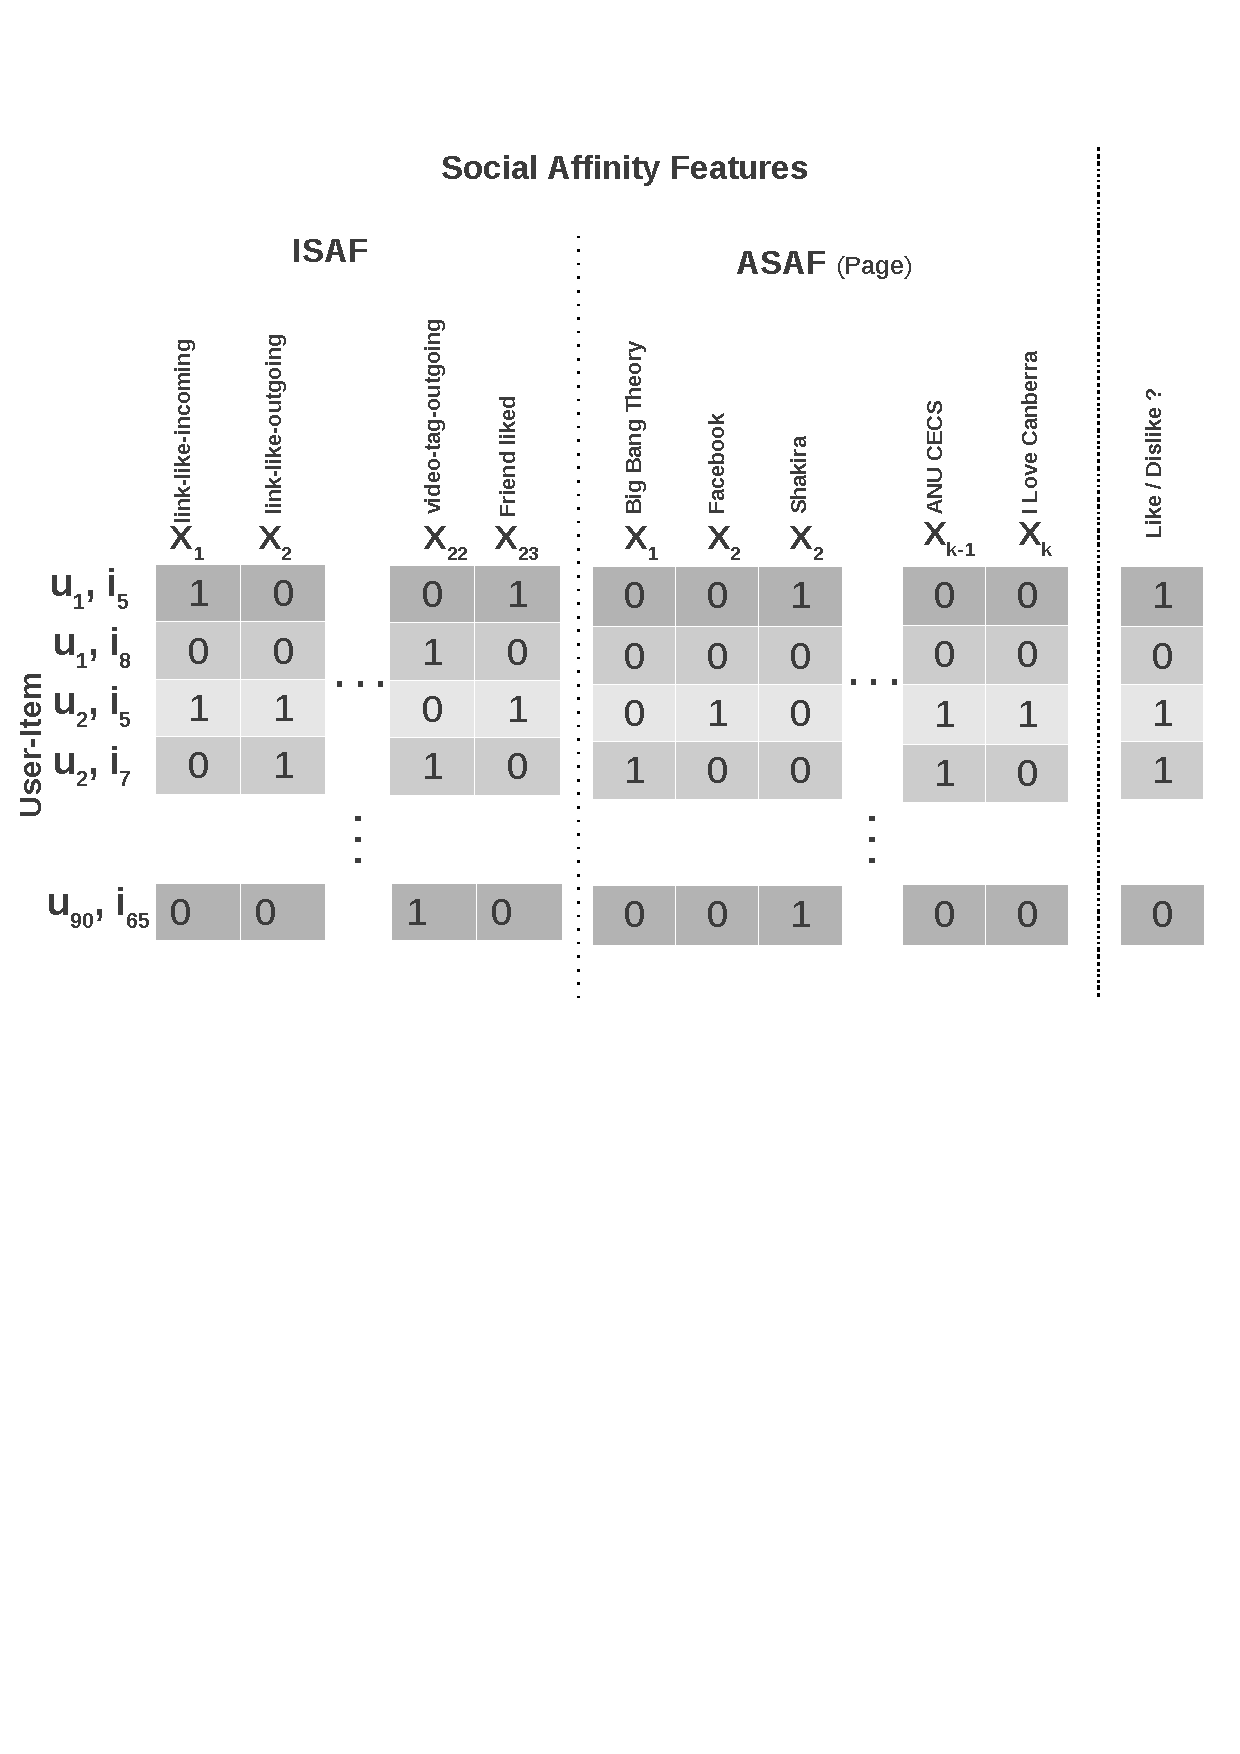
\includegraphics[width=1\linewidth]{data/plots/features/saf_features}
\caption{SAF training data example: each row corresponds to a training
  data sample for a specific user-item pair $(u,i)$ for which the
  prediction target $\like(u,i)$ is observed (last column).  All other
  columns represent the value of ISAF or ASAF features
  evaluated relative to the $(u,i)$ label of each row.
  All columns are binary-valued ($0=\false,1=\true$).}
\label{fig:features_overview}
\end{figure}
%#suvash#
%%%%%%%%%%%%%%%%%%%%%%%%%%%%%%%%%%%%%%%%%%%%%%%%%%%%%%%%%%%%%%%%%%%%%%

To understand how SAF works, it helps to visualise the training data as shown
in Fig~\ref{fig:features_overview}.  

\subsection{SAF vs. Other Filtering Methods}

While a classification approach to recommendation might evoke
comparisons to \emph{content-based filtering} (CBF)~\cite{newsweeder},
we remark that CBF is not a \emph{social} recommendation approach and
unlike CBF, SAF does not require explicit user features (e.g., age,
gender, location, etc.) or item descriptors (link text, link genre,
etc.); in contrast, SAF uses interaction and/or activity data for
social network users to define SAGs and learns the affinities between
a user (ego) and the different set of alters as defined by these SAGs.
Additionally, unlike state-of-the-art \emph{social collaborative filtering} 
approaches~\cite{socinf,rrmf,ste,sorec,sr,Noel2012NOF,lla}, SAF does
not aggregate user-user interaction and shared activity data into a
single aggregate statistic, instead it uses fine-grained distinctions
in this social data to define a large number of SAGs and learns which
of these SAGs are informative for recommendation.




\section{Evaluation}

\subsection{Data Description}
\label{sec:datadesc}


We built a Facebook App\footnote{Name and link omitted
for anonymity.} to collect information about users, 
their interactions and preferences.  
%data about Facebook users and their Facebook friends
%are collected through our Facebook App. 
Our dataset contains information about each App user, along with a
subset of information about their friends visible to the App.  The
data collection is performed with full permission from the user and in
accordance with an approved Ethics Protocol\footnote{Link omitted for
anonymity.}.

Over 200 users installed the Facebook App sometime during the
evaluation period. At any time, around 100 users have actively used
the App. From these core App users, the App has access to their
detailed Facebook profiles and their interactions with a total of
39,850 friends.
%interaction data.  
While we have complete interaction data for the App
users with their friends, and profile data (including
wall post data) for the App users and friends, we do not have complete
interactions for the App users' friends (unless they themselves are
App users).  Hence in the forthcoming analysis, we limit our
evaluation to App users for which we are assured to have full
interaction data.

Our App tracks many user (and their friends') details and interactions
on Facebook.  Interactions that occur through wall posts provide a
rich variety of content and interaction data.  We distinguish four
Facebook items from wall posts: general posts (e.g., status updates,
activity updates such as new friends, and interactions such as the
user liked these pages), links, photos and videos. Four main
interactions on these items are permitted by Facebook: posting an item
to a friend's wall, commenting, liking, and tagging\footnote{Some
Facebook interaction features such as liking comments were introduced
after App user studies began and so are not tracked.}.  The App does
not track deletions of these items and interactions (e.g., unlike) for
performance reasons and we found very few deletions during an initial
testing stage.

%% Scott edited up to this point: please don't undo unless something
%% stated is incorrect.  We cannot use the name LinkR b/c it reveals
%% who we are.  I deleted some details of the ethics protocol as they
%% are not needed in this submitted version of the paper for review,
%% can add in camera-ready if needed.  Changed object -> item to be
%% consistent with later terminology.

%% Nguyen: please edit from this point on, only including statistics
%% that are relevant to data shown in the various plots, plus age
%% info as well (since this is useful to know).  So for example, 
%% you can comment out all non-gender, non-age demographics (locale, 
%% location, etc.) as well as unused table data (e.g., note that *only*
%% education and school -- first two rows of Table 3 are needed).
%% SVN has the record if we ever need to add this data back in.
%%
%% I did a search replace of LinkR with App... need to fix some 
%% awkward mentions.
%%
%% In short make sure all data mentioned is relevant to evaluation
%% section, other information is superfluous.

We summarize relevant basic statistics of the data in Table~\ref{tab:interactions}-\ref{tab:interests} below.
The tables distinguish the data from the App users and from
all App users and friends. Table~\ref{tab:interactions}
summarizes the number of records for each item (row) and interaction (column)
combination. Table~\ref{tab:demographics} shows 
some demographics from user profiles\footnote{Note that
count of schools are not unique as each user can attend more than one
degree of the same type.}.

\begin{table}
\centering
\begin{tabular}{|>{\small}l|>{\small}r|>{\small}r|>{\small}r|>{\small}r|}
\hline
\textbf{App Users} & \textbf{Posts} & \textbf{Tags} & \textbf{Comments} & \textbf{Likes} \\
\hline
\textbf{Wall} & 36,359 & 7,711 & 22,388 & 15,999 \\
\hline
\textbf{Link} & 5,304 & --- & 7,483 & 6,566 \\
\hline
\textbf{Photo} & 4,933 & 28,341 & 10,976 & 8,612 \\
\hline
\textbf{Video} & 245 & 2,525 & 1,970 & 843 \\
\hline
\hline
\textbf{App Users} & \textbf{Posts} & \textbf{Tags} & \textbf{Comments} & \textbf{Likes} \\
\textbf{and Friends} & & & & \\
\hline
\textbf{Wall} & 4,301,306 & 1,215,382 & 3,122,019 & 1,887,497 \\
\hline
\textbf{Link} & 678,612 & --- & 891,986 & 995,214 \\
\hline
\textbf{Photo} & 1,268,816 & 9,620,708 & 3,431,321 & 2,469,859 \\
\hline
\textbf{Video} & 59,244 & 904,604 & 486,677 & 332,619 \\
\hline
\end{tabular}
\caption{Number of records in Items and Interactions Tables. Rows are type of Facebook item and columns are type of Facebook interaction.}
\label{tab:interactions}
\end{table}


\begin{table}
\centering
\begin{tabular}{|>{\small}l|>{\small}r|>{\small}r|}
\hline
\textbf{Table} & \textbf{\#Records} & \textbf{\#Records} \\
& \textbf{(App Users)} & \textbf{(App User} \\
& & \textbf{and Friends)} \\
\hline
Users & 119 & 38,378 \\
\hline
\hline
\textbf{Column} & \textbf{\#Non-empty} & \textbf{\#Non-empty} \\
& \textbf{(App Users)} & \textbf{(App User} \\
& & \textbf{and Friends)} \\
\hline
Gender & 118 & 37,872 \\
%\hline
%Locale & 103 & 36,900 \\
%\hline
%Timezone & 103 & 117 \\
\hline
Birthday & 118 & 28,633 \\
%\hline
%Hometown\par Location & 63 & 17,584 \\
%\hline
%Current\par Location & 71 & 20,088 \\
\hline
\hline
\textbf{Breakdown} & \textbf{Count} & \textbf{Count} \\
& \textbf{(App Users)} & \textbf{(App User} \\
& & \textbf{and Friends)} \\
\hline
Male & 85 & 20,840 \\
\hline
Female & 33 & 17,032 \\
\hline
%High School & 104 & 29,503 \\
%\hline
%College & 115 & 29,223 \\
%\hline
%Graduate School & 56 & 7733 \\
%\hline
%%lexing: isn't it just "College" and not "Degree:College"
%Degree:\par High School & 104 & 29,503 \\
%\hline
%Degree:\par College & 115 & 29,223 \\
%\hline
%Degree:\par Graduate School & 56 & 7733 \\
%\hline
\end{tabular}
\caption{App user demographics.}
\label{tab:demographics}
\end{table}

\begin{table}
\centering
\begin{tabular}{|>{\small}l|>{\small}r|>{\small}r|}
\hline
\textbf{Table} & \textbf{\#Records} & \textbf{\#Records} \\
& \textbf{(App Users)} & \textbf{(App User} \\
& & \textbf{and Friends)} \\
%\hline
%Activities & 394 & 92,148 \\
%\hline
%Books & 266 & 52,690 \\
%\hline
%Favorite Athletes & 58 & 23,009 \\
%\hline
%Favorite Teams & 35 & 14,772 \\
\hline
Groups & 3,469 & 373,608 \\
\hline
Page Likes & 10,771 & 825,452 \\
\hline
Favourites & 4,284 & 892,820\\
%\hline
%Inspirational People & 39 & 7,815 \\
%\hline
%Interests & 153 & 36,085 \\
%\hline
%Movies & 616 & 149,197 \\
%\hline
%Music & 1,245 & 318,296 \\
%\hline
%Sports & 48 & 8,663 \\
%\hline
%Television & 819 & 144,308 \\
\hline
\end{tabular}
\caption{Groups of Interests Tables}
\label{tab:interests}
\end{table}

\begin{table}
\centering
\begin{tabular}{|>{\small}l|>{\small}r|>{\small}r|}\hline
&\textbf{Friend}  & \textbf{Non-Friend} \\
&\textbf{recommendation}  & \textbf{recommendation} \\
\hline
Like& 1392 & 1127 \\
\hline
Dislike& 895 & 2111\\
\hline
\end{tabular}
\caption{Datas breakdown by friend/non-friend and like/dislike}
\end{table}


\begin{table}
\centering
\begin{tabular}{|c|c|}
\hline
 Favourite & \# items \\
\hline
        Activities  &     228 \\
  FavoriteAthletes  &      57 \\
             Books  &     126 \\
         Interests  &      92 \\
            Movies  &     360 \\
             Music  &     671 \\
            Sports  &      12 \\
     FavoriteTeams  &      28 \\
        Television  &     361 \\
\hline
\end{tabular}
\caption{Favourite item counts}
\end{table}

\subsection{SAF Analysis}
\label{sec:saf_analysis}

%%%%%%%%%%%%%%%%%%%%%%%%%%%%%%%%%%%%%%%%%%%%%%%%%%%%%%%%%%%%%%%%%%%%%%%%%%%
\begin{figure*}[tbp!]
%\centering
\hspace{-6mm}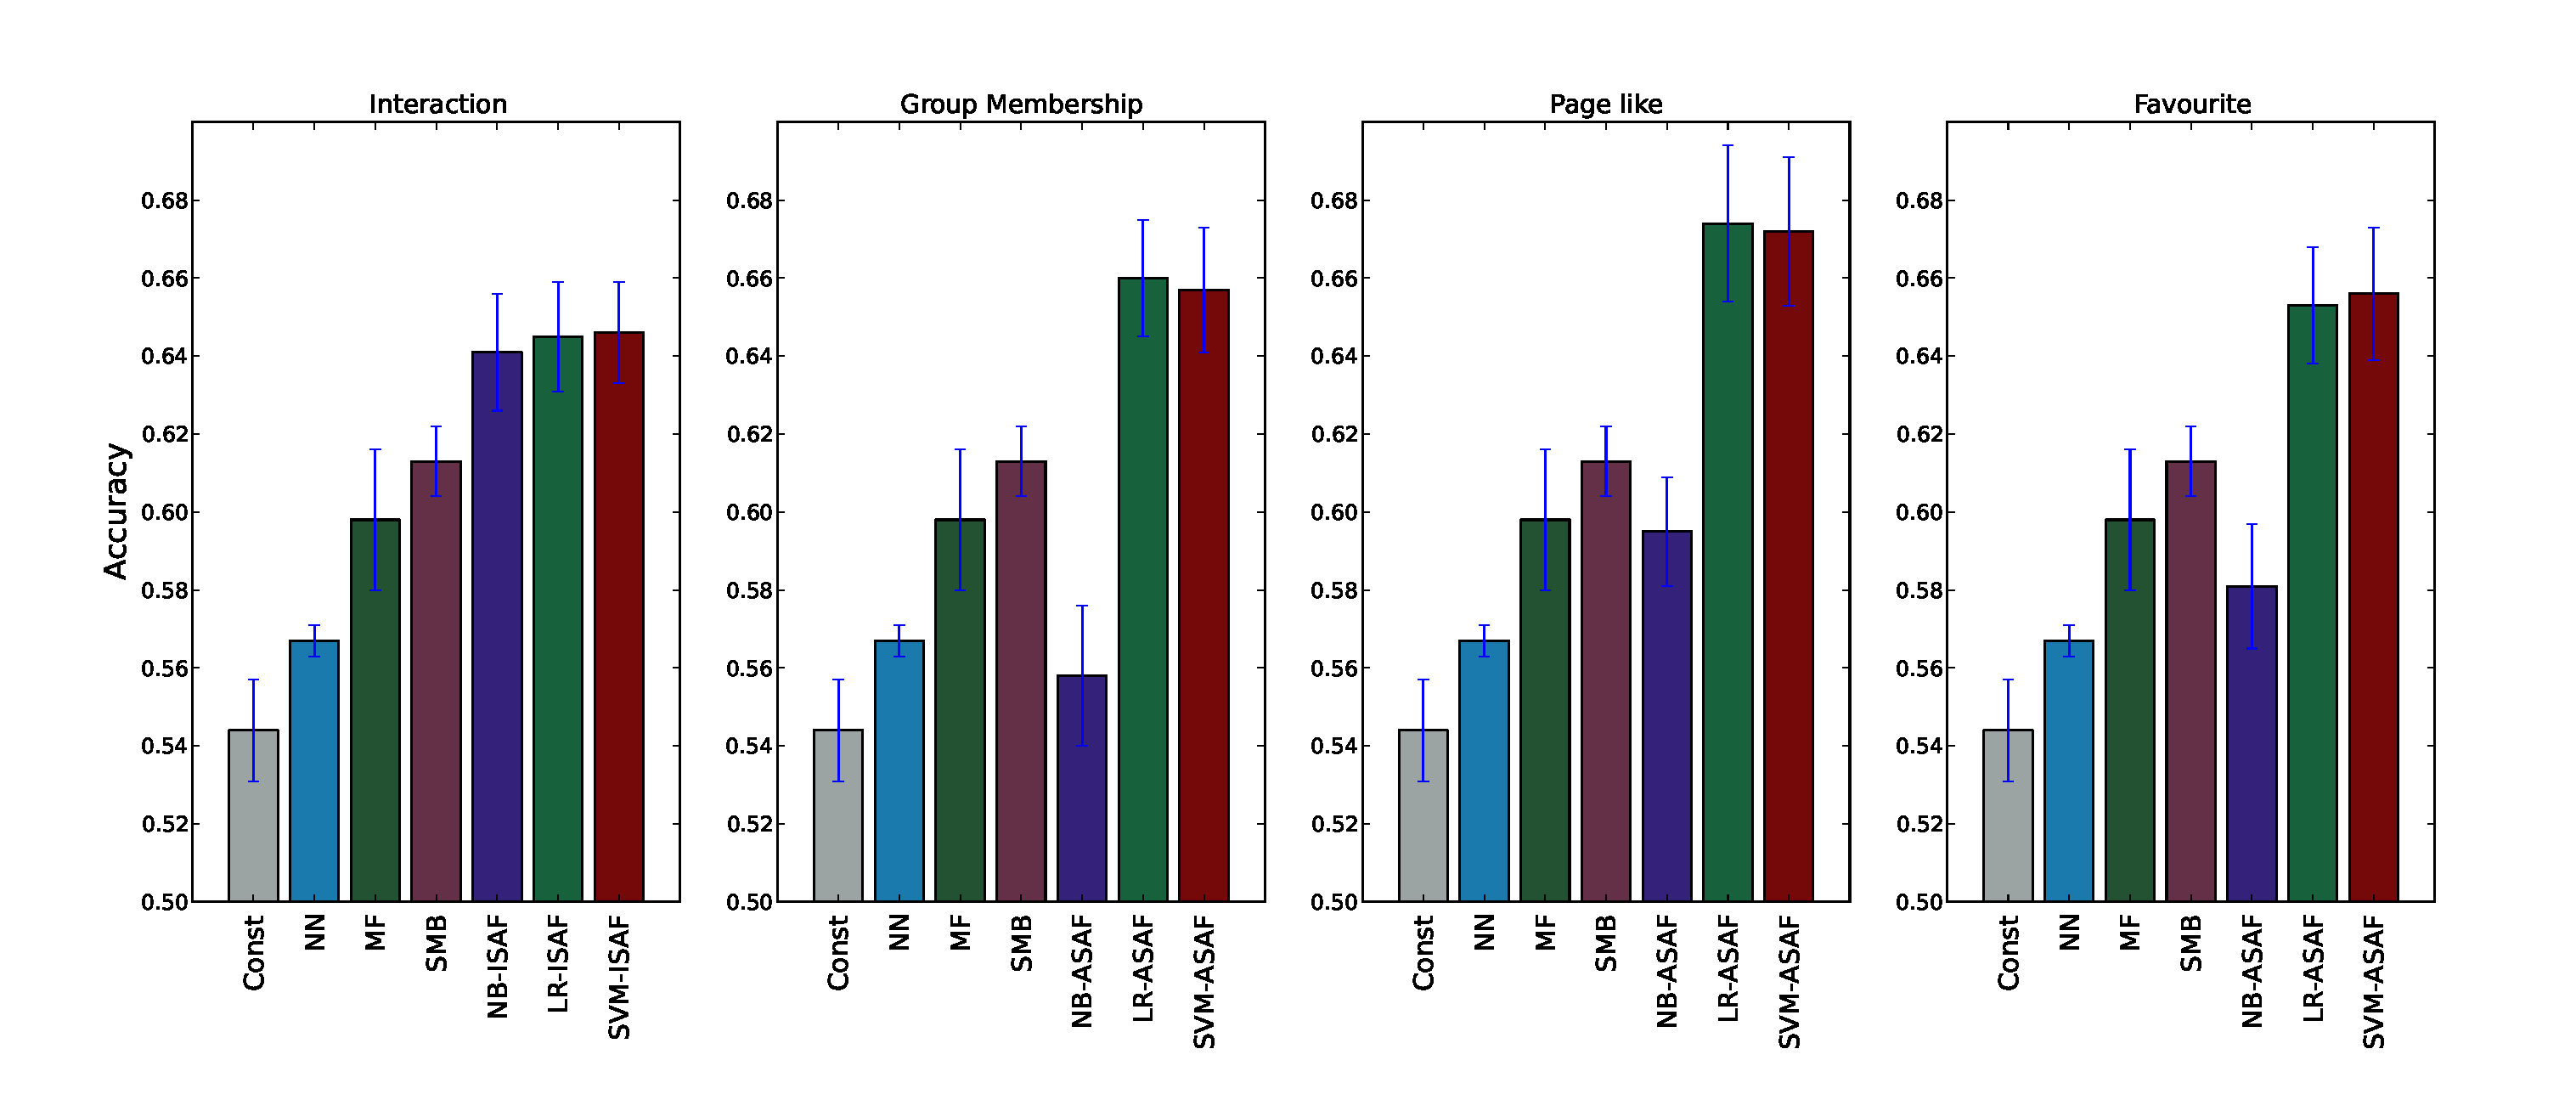
\includegraphics[width=190mm, height=100mm]{data/plots/accuracy/accuracyLargeNew.eps}
\caption{ {\bf TODO: update caption and make more verbose to explain major take-home points of figures -- reviewers will just skim among figures to get key points.  Likewise for later captions.}  Accuracy of predictors (constant, social matchbox, naive bayes, logistic regression, SVM) for Interaction and Activity  features }
\label{Fig1}
\end{figure*}
%%%%%%%%%%%%%%%%%%%%%%%%%%%%%%%%%%%%%%%%%%%%%%%%%%%%%%%%%%%%%%%%%%%%%%%%%%%

{\bf TODO: first need to clearly outline and label all baseline algorithms
           and all novel algorithms... see how this was done in experimental
           section of WWW-12 paper.}

{\bf TODO: make clear some baselines are standard CF (NN, MF), some are social CF -- also explain
           briefly what social Matchbox is.}

{\bf TODO: clarify what the error bars are showing and how
           cross-validation was performed.}

Fig \ref{Fig1} compares the accuracies of constant predictor and
social matchbox with SAF based on na\"{i}ve Bayes, logistic regression
and SVM classification for a range of interaction and activity (group,
page, favourite) SAGs.  In all of our experiments SAF variants
performed significantly better than Social Matchbox and the constant
predictor except for na\"{i}ve Bayes, we conjecture this is due to the
correlations between SAGs that cause na\"{i}ve Bayes to over- or
under-estimate the true probability of likes.

In general we note in Fig \ref{Fig1} that activities appear to be
more predictive than interactions, but we believe the reasons for this
are quite simple: Interaction SAGs can only evaluate the friends of
user $u$ whereas Activity SAGs are able to look at all users,
independent of $u$'s friends.
Hence, given the general sparsity of ``likes'' data in Facebook, 
Activity SAGs appear to draw on a much larger group of SAGs
with much more activity.

Among activities, Fig \ref{Fig1} shows that activities are more
predictive than interactions. Among the activities, page likes are the
most predictive followed by group membership and favourites.
Returning to our conjecture that data sparsity can hurt SAF, we note
from Table~\ref{tab:interests} that page likes are more prevalent than
groups and favourites.  Moreover, these results may indicate that
there is more social affinity between co-members of inherently social
activities like groups and pages than between users who simply have
favourites in common.

Comparing SAF to the state-of-the-art in social
collaborative filtering (SCF) as represented by Social
Matchbox~\cite{Noel2012NOF}, we observe that SAF consistently
outperforms it.  We note that the key difference of SAF vs. SCF is
that SAF exploits the predictiveness of fine-grained interactions ---
it breaks down into groups, whereas most SCF
approaches~\cite{Noel2012NOF,lla,socinf,sr,rrmf,sorec,ste} is that
instead of collapsing a diverse set of interactions into aggregate
statistics such as the number of interactions between user $u_1$ and
user $u_2$, regardless of whether $u_1$ tagged $u_2$ in a photo or
$u_1$ liked a photo on $u_2$'s wall.  Clearly there is a great deal of
benefit deriving from the fine-grained interactions indicating why
without modeling any latent space and using a simple linear
classifier, SAF can outperform SCF methods based on matrix
factorization approaches that attempt to learn latent user and item
features.

On two final notes, we remark that SAF yields a computational and
optimization advantage over SCF in that it is straightforward and
efficient to find a globally optimal classifier with respect to certain training
criteria (e.g., optimising log loss in logistic regression or hinge
loss in SVMs) unlike SCF approaches that generally rely on
computationally expensive matrix factorization techniques that lack
optimality guarantees.  Further, we also note quite surprisingly that
SAF inherently scales to a large number of users and generalizes to
completely new users without suffering from the cold-start problem:
this is simply because nothing SAF learns is user dependent, it learns
to weight SAGs independent of any particular user.

Given the clearly demonstrated benefits of SAF, we now proceed in the
next two sections to analyse the two primary types of SAG features
(interactions and activities) to better understand characteristics of
both informative and uninformative SAGs in each context and the social
phenomena that may be responsible for these characteristics.


\subsection{Interaction Analysis}
\label{sec:interaction_analysis}

%%%%%%%%%%%%%%%%%%%%%%%%%%%%%%%%%%%%%%%%%%%%%%%%%%%%%%%%%%%%%%%%%%%%%%%%%%%
\begin{table}
\caption{Conditional entropy of various interactions.}
\label{table:ce_interaction}
\vspace{-2mm}
\centering
{\footnotesize
	\begin{tabular}{| >{\small}l | >{\small}r | }
		\hline
		\textbf{ Modality ($X$)} & $H(Y|X=true)$ \\
		\hline
		{ video } & 0.850 \\
		\hline
		{ link } & 0.915 \\
		\hline
		{ post } & 0.918 \\
		\hline
		{ photo } & 0.926 \\
		\hline
\multicolumn{2}{c}{}\\
		\hline
		\textbf{ Type ($X$)}  & $H(Y|X=true)$ \\
		\hline
		{ tags }  &  0.920 \\
		\hline
		{ comments }  &  0.921 \\
		\hline
		{ likes }  &  0.924 \\
		\hline
\multicolumn{2}{c}{}\\
		\hline
		\textbf{ Direction ($X$) } & $H(Y|X=true)$ \\
		\hline
		{ outgoing }  &  0.928 \\
		\hline
		{ incoming }  &  0.935 \\
		\hline
\multicolumn{2}{c}{}\\
%	\end{tabular}
%\end{table*}
%%%%%%%%%%%%%%%%%%%%%%%%%%%%%%%%%%%%%%%%%%%%%%%%%%%%%%%%%%%%%%%%%%%%%%%%%%%
%	
%%%%%%%%%%%%%%%%%%%%%%%%%%%%%%%%%%%%%%%%%%%%%%%%%%%%%%%%%%%%%%%%%%%%%%%%%%%
%\begin{table*}
%%	\begin{tabular}{| >{\small}l | >{\small}r |}
%		\hline
%		\textbf{Modality-Direction} ($X$) & $H(Y|X=true)$ \\
%		\hline
%		tags-outgoing & 0.885 \\
%		likes-outgoing & 0.885 \\
%		tags-incoming & 0.900 \\
%		likes-incoming & 0.902 \\
%		comments-outgoing & 0.908 \\
%		comments-incoming & 0.912 \\
%		\hline
%	\end{tabular}
%%\multicolumn{2}{c}{}\\
%	\begin{tabular}{| >{\small}l | >{\small}r |}
                \hline	
		\textbf{Action-Direction} ($X$) & $H(Y|X=true)$ \\
		\hline
		photo-outgoing & 0.857 \\
		video-outgoing & 0.863 \\
		link-outgoing & 0.895 \\
		link-incoming & 0.896 \\
		post-incoming & 0.902 \\
		post-outgoing & 0.906 \\
		video-incoming & 0.915 \\
		photo-incoming & 0.921 \\
		\hline
				
	\end{tabular}}
\end{table}
%%%%%%%%%%%%%%%%%%%%%%%%%%%%%%%%%%%%%%%%%%%%%%%%%%%%%%%%%%%%%%%%%%%%%%%%%%%

%%%%%%%%%%%%%%%%%%%%%%%%%%%%%%%%%%%%%%%%%%%%%%%%%%%%%%%%%%%%%%%%%%%%%%%%%%%
\begin{figure*}[tbp!]
\centering
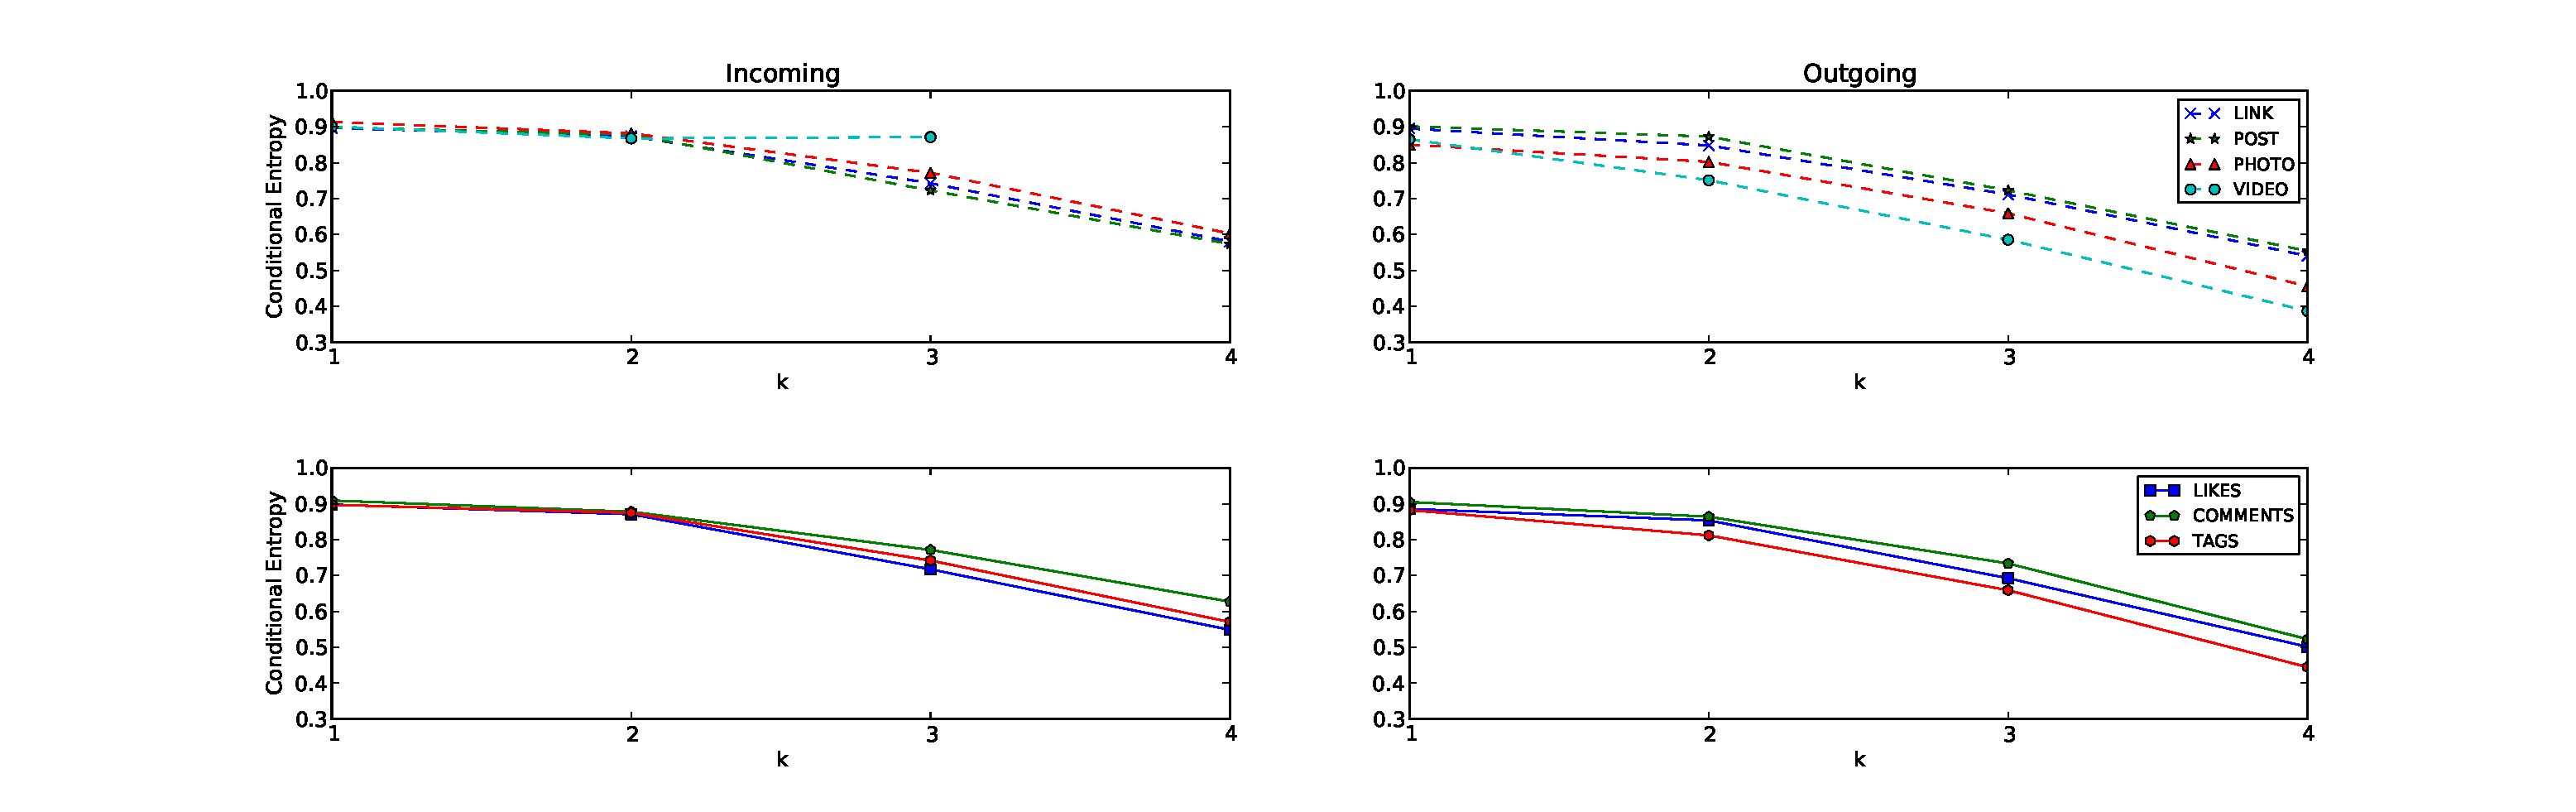
\includegraphics[width=200mm]{data/plots/vsk/ModalityActionsvsKFriends.eps}
\caption{Conditional Entropy  of modalities/activities for incoming/outgoing interactions vs item liked by atleast k friends}
\label{Fig2}
\end{figure*}
%%%%%%%%%%%%%%%%%%%%%%%%%%%%%%%%%%%%%%%%%%%%%%%%%%%%%%%%%%%%%%%%%%%%%%%%%%%

\section{Interaction Analysis}

In this section we analyze Interaction SAGS, namely those SAGs that
are built w.r.t. a user $u$'s interactions.  Recalling our Methodology,
we have three distinctions for user interactions: modality, action,
and directionality.  First we analyze various interactions individually
and jointly to understand what interactions define SAGs with a high
social affinity for a user $u$'s preferences.  To this end, we make a few
observations from Table~\ref{table:ce_interaction}: 
\begin{itemize}
\item Users seem to have a stronger preferential affinity with
those they interact with on videos vs. other modalities.  This could
be due to the fact that video viewing is time-consuming and users
inherently only watch the videos of those whose preferences they
often share.
\item Tagging has a slightly better conditional entropy than commenting
and liking indicating that tagging is a sign of a strong social tie.~\cite{***}
\item A user is more likely to share preferences with someone who she
initiates the interaction with (outgoing) vs. with someone who initiates
the interaction with her (incoming).~\cite{saez2011high}
\end{itemize}

In figure \ref{Fig2} we plot conditional entropy of modality and
action for incoming/outgoing interactions constrained to links
liked by at least $k$ friends in the SAG.  Figure \ref{Fig2} reiterates
many comments made above for various $k$.  In addition, we note that
%\begin{itemize}
%% NOTED ABOVE NOW
%  \item Some interactions are more predictive than other. For
%    eg. videos and photo interactions were found to be significantly
%    more predictive than post and link interactions. Similarly,
%    tagging action is often more predictive than commenting and
%    liking.
%  \item As noted by previous work~\cite{saez2011high}, we observe that
%    outgoing interactions are more predictive than incoming
%    interactions. Furthermore, the differentiation between
%    predictiveness modalities and actions is more pronounced in
%    outgoing interactions than in incoming interactions.
%  \item 
preference affinity with a SAG increases as more people in the SAG
like the item --- then the more likely a user is to like an item.
While incoming interactions were not as predictive as outgoing
interactions for the same $k$, we note that higher $k$ for an incoming
interaction can be more predictive than lower $k$ for an outgoing
interaction.  This exhibits repeated exposure properties of epidemic
models for social networks~\cite{Golub2010selectionbiase}.
%\end{itemize}




\subsection{Activity Analysis}
\label{sec:activity_analysis}

%!TEX root = document.tex

% Note: activity SAGs can go beyond friends.

In this section we evaluate the correlation between the conditional
entropy and size of groups, pages and favourites.

Fig \ref{Fig3} shows the relationship between conditional
    entropy and logistic regression weights versus the size of activity
    groups. Here the size of a {\em group}, {\em page} and {\em favorite} 
    is the number of total users in the activity group. 
    For {\em Pages} and {\em Favorites} this is the total number of Facebook users, 
    whether or not they are in the App users' ego network, while for 
    {\em Groups} only the number of users in the App users' ego network is visible to our app.
    Both scatter plots shows that the activity groups of small size can be
    highly predictive (low conditional entropy or weights that deviate
    extremely from zero) whereas large groups are rarely predictive.

In \ref{Fig4} we plot the average conditional entropy of the top
    10\% of features cumulative up to the size of the activity group given on the
    x-axis; this allows us to determine the marginal contribution of
    larger groups to the average conditional entropy as larger groups
    are incrementally added in.  This graph 
    distinctly shows that the small sizes of groups, pages and favourites
    have low average conditional entropy that transitions sharply to a
    higher average once a size threshold has been met.  From 
    Fig~\ref{Fig4} we can infer that the group sizes up to 50 and
    page/favourite sizes up to $10^{5}$ are most predictive.

{\bf TODO: make this consistent with earlier discussion regarding persistence,
temporally sychronized.}

 We also analyze predictiveness of favourites by categories in
    Fig~\ref{Fig5}. It shows that SAGs consisting of shared interests,
    activity, television, and books are on average most predictive, while 
    music, movies, favourite teams, sports and athletes are on average
    least predictive.  While favourite teams, sports and athletes may be
    too focused to offer much predictiveness vs. the other more diverse
    categories, it is interesting that movies and music favourites
    are not very predictive on average.  This may have to do with the fact that
    these are typically ephemeral favourites that may be heavily influenced
    by popularity as opposed to true personal preference.
%\end{itemize}

%In Fig~\ref{Fig4} we plot the average conditional entropy of top
%    10\% features cumulative over the size of activity group. It
%    distinctly shows that the small sized group, pages and favourites
%    have low average conditional entropy. Furthermore, it explains
%    average conditional entropy decreases as size increases. From the
%    figure \ref{Fig4} we can infer that the group size upto 50 and
%    page/favourite size upto $10^{5}$ can be highly predictive.
%
%We also analyze predictiveness of favourites by categories in
%    Fig \ref{Fig5}. It shows that television, books, music and movies
%    are predictive whereas favourite teams, sports and athletes are
%    less predictive.
%\end{itemize}


%%%%%%%%%%%%%%%%%%%%%%%%%%%%%%%%%%%%%%%%%%%%%%%%%%%%%%%%%%%%%%%%%%%%%%%%%%%
\begin{figure*}[tbp!]
\centering
\begin{tabular}{ccc}
\begin{tabular}{ccc}
\subfloat[Fig:][]{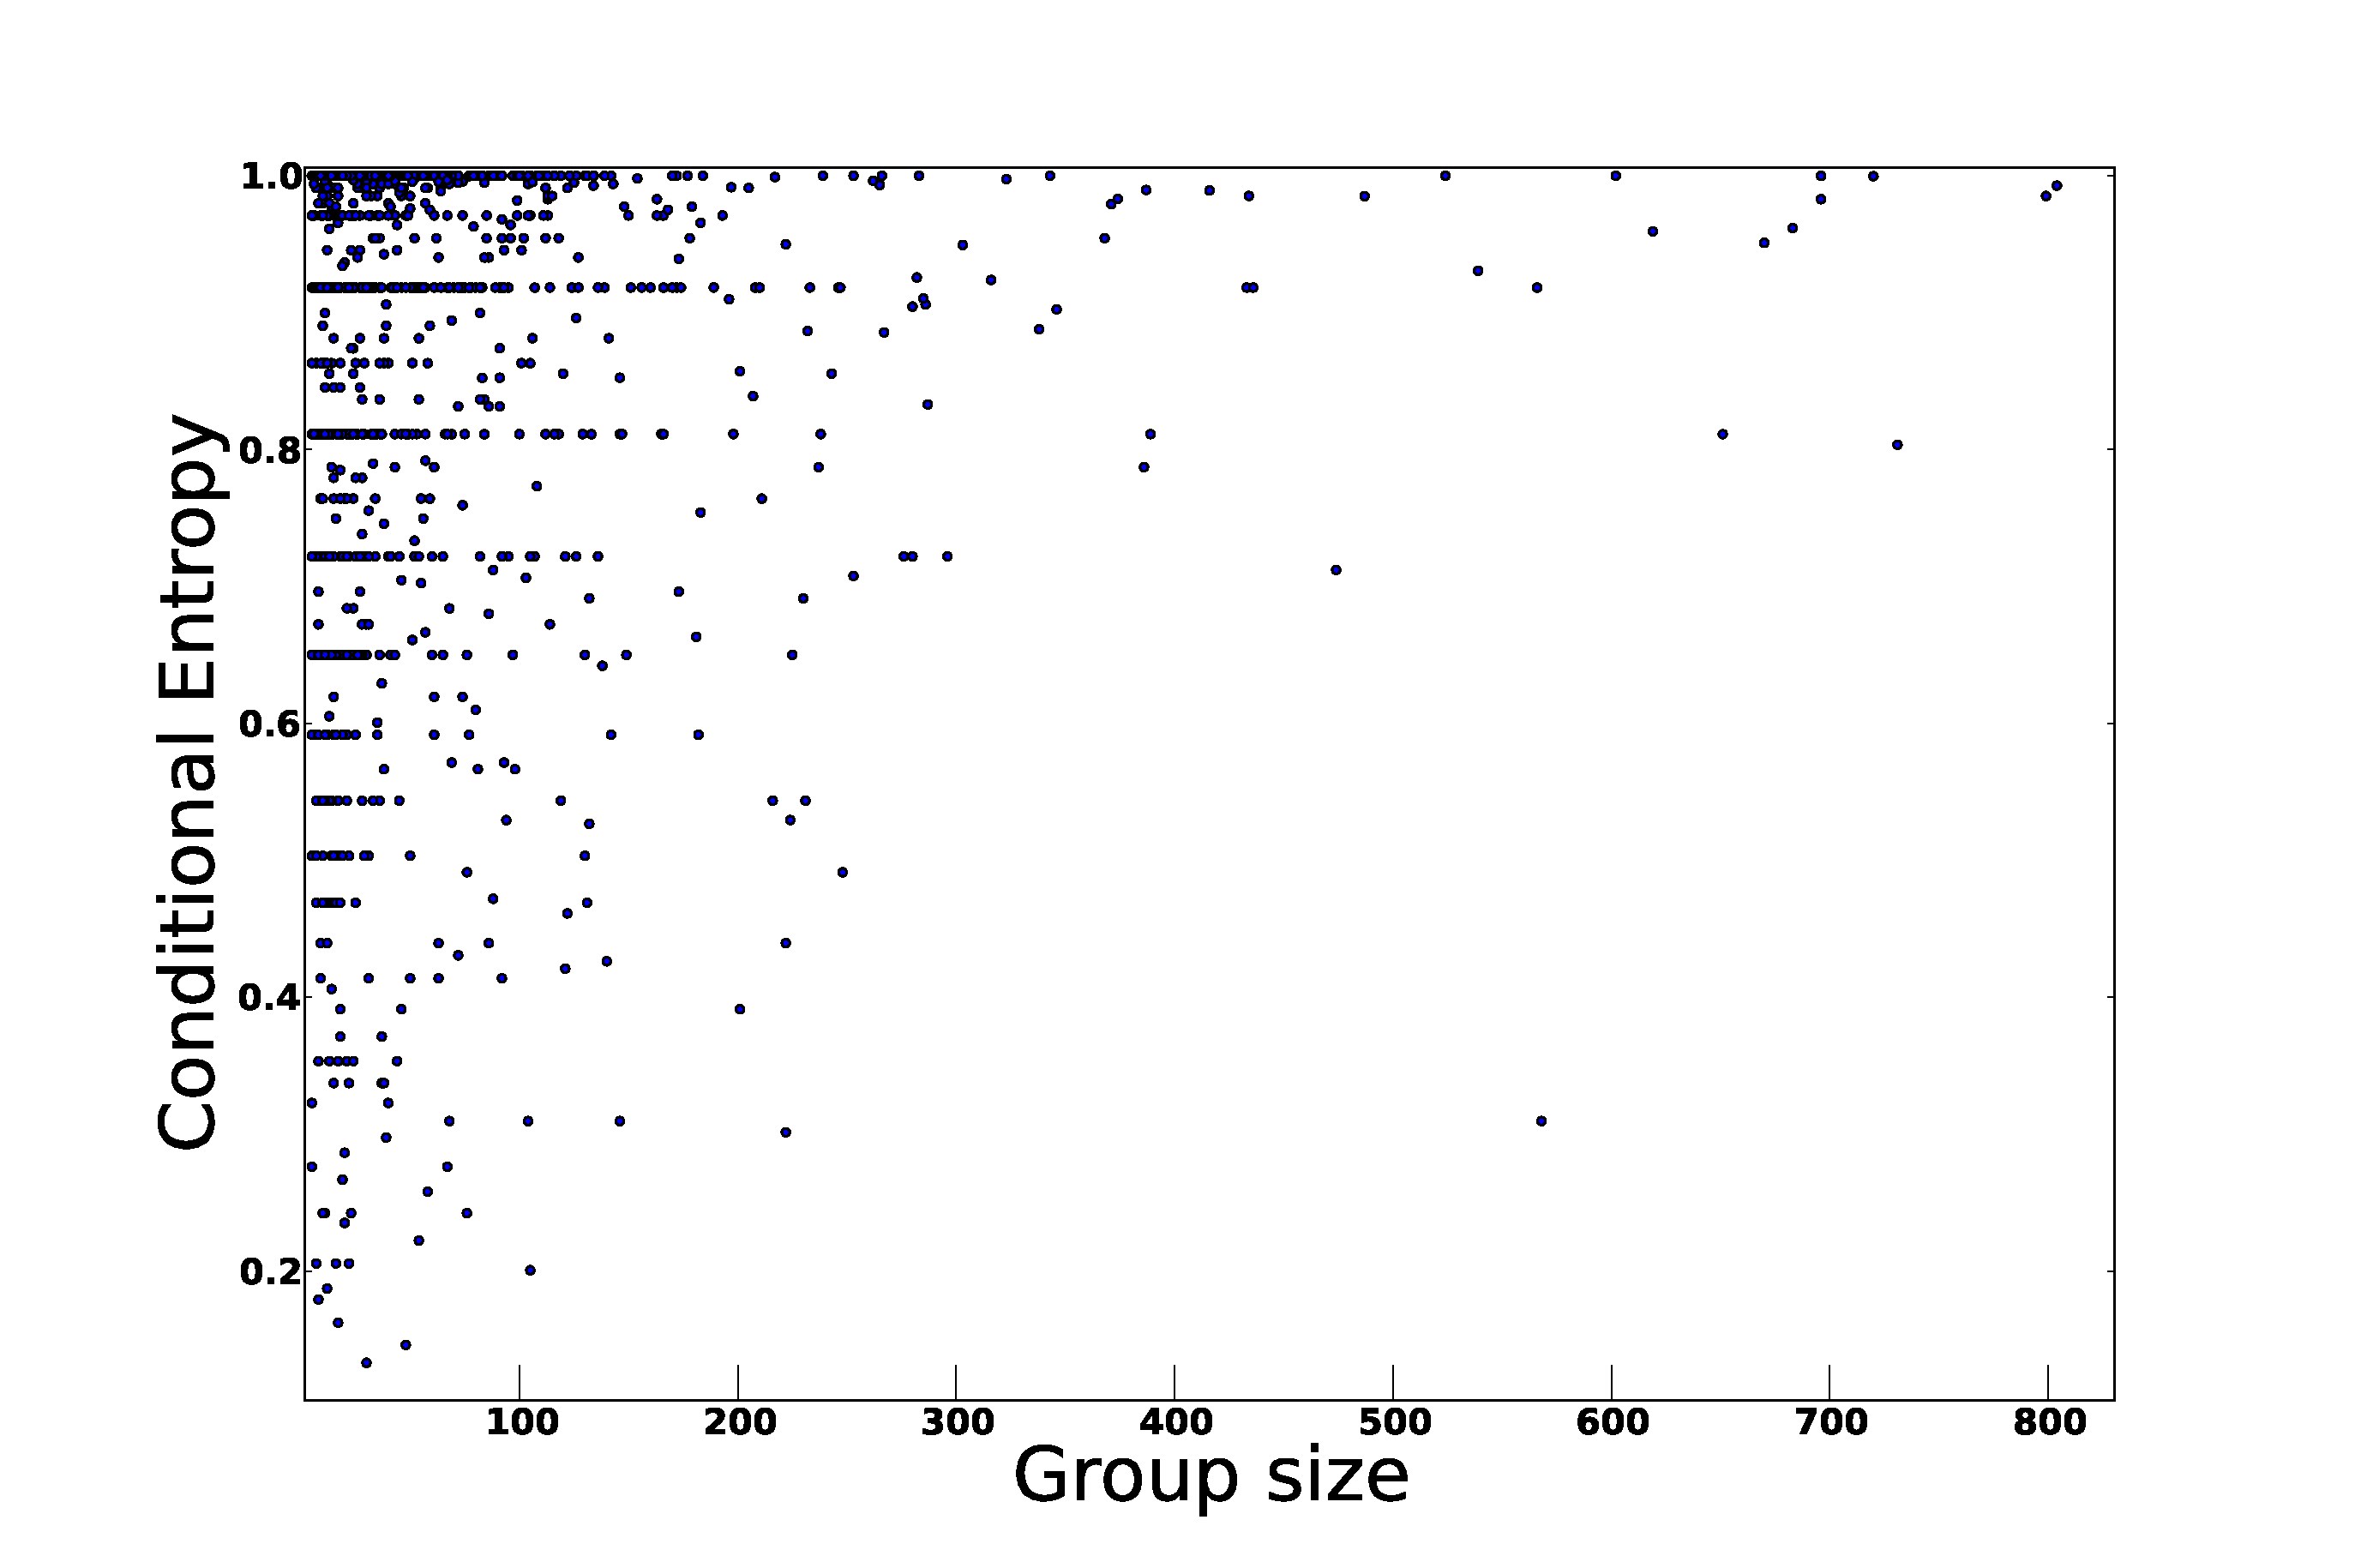
\includegraphics[width=45mm, height=35mm]{data/plots/new/CEvsGroupSize.eps}}
\subfloat[Fig:][]{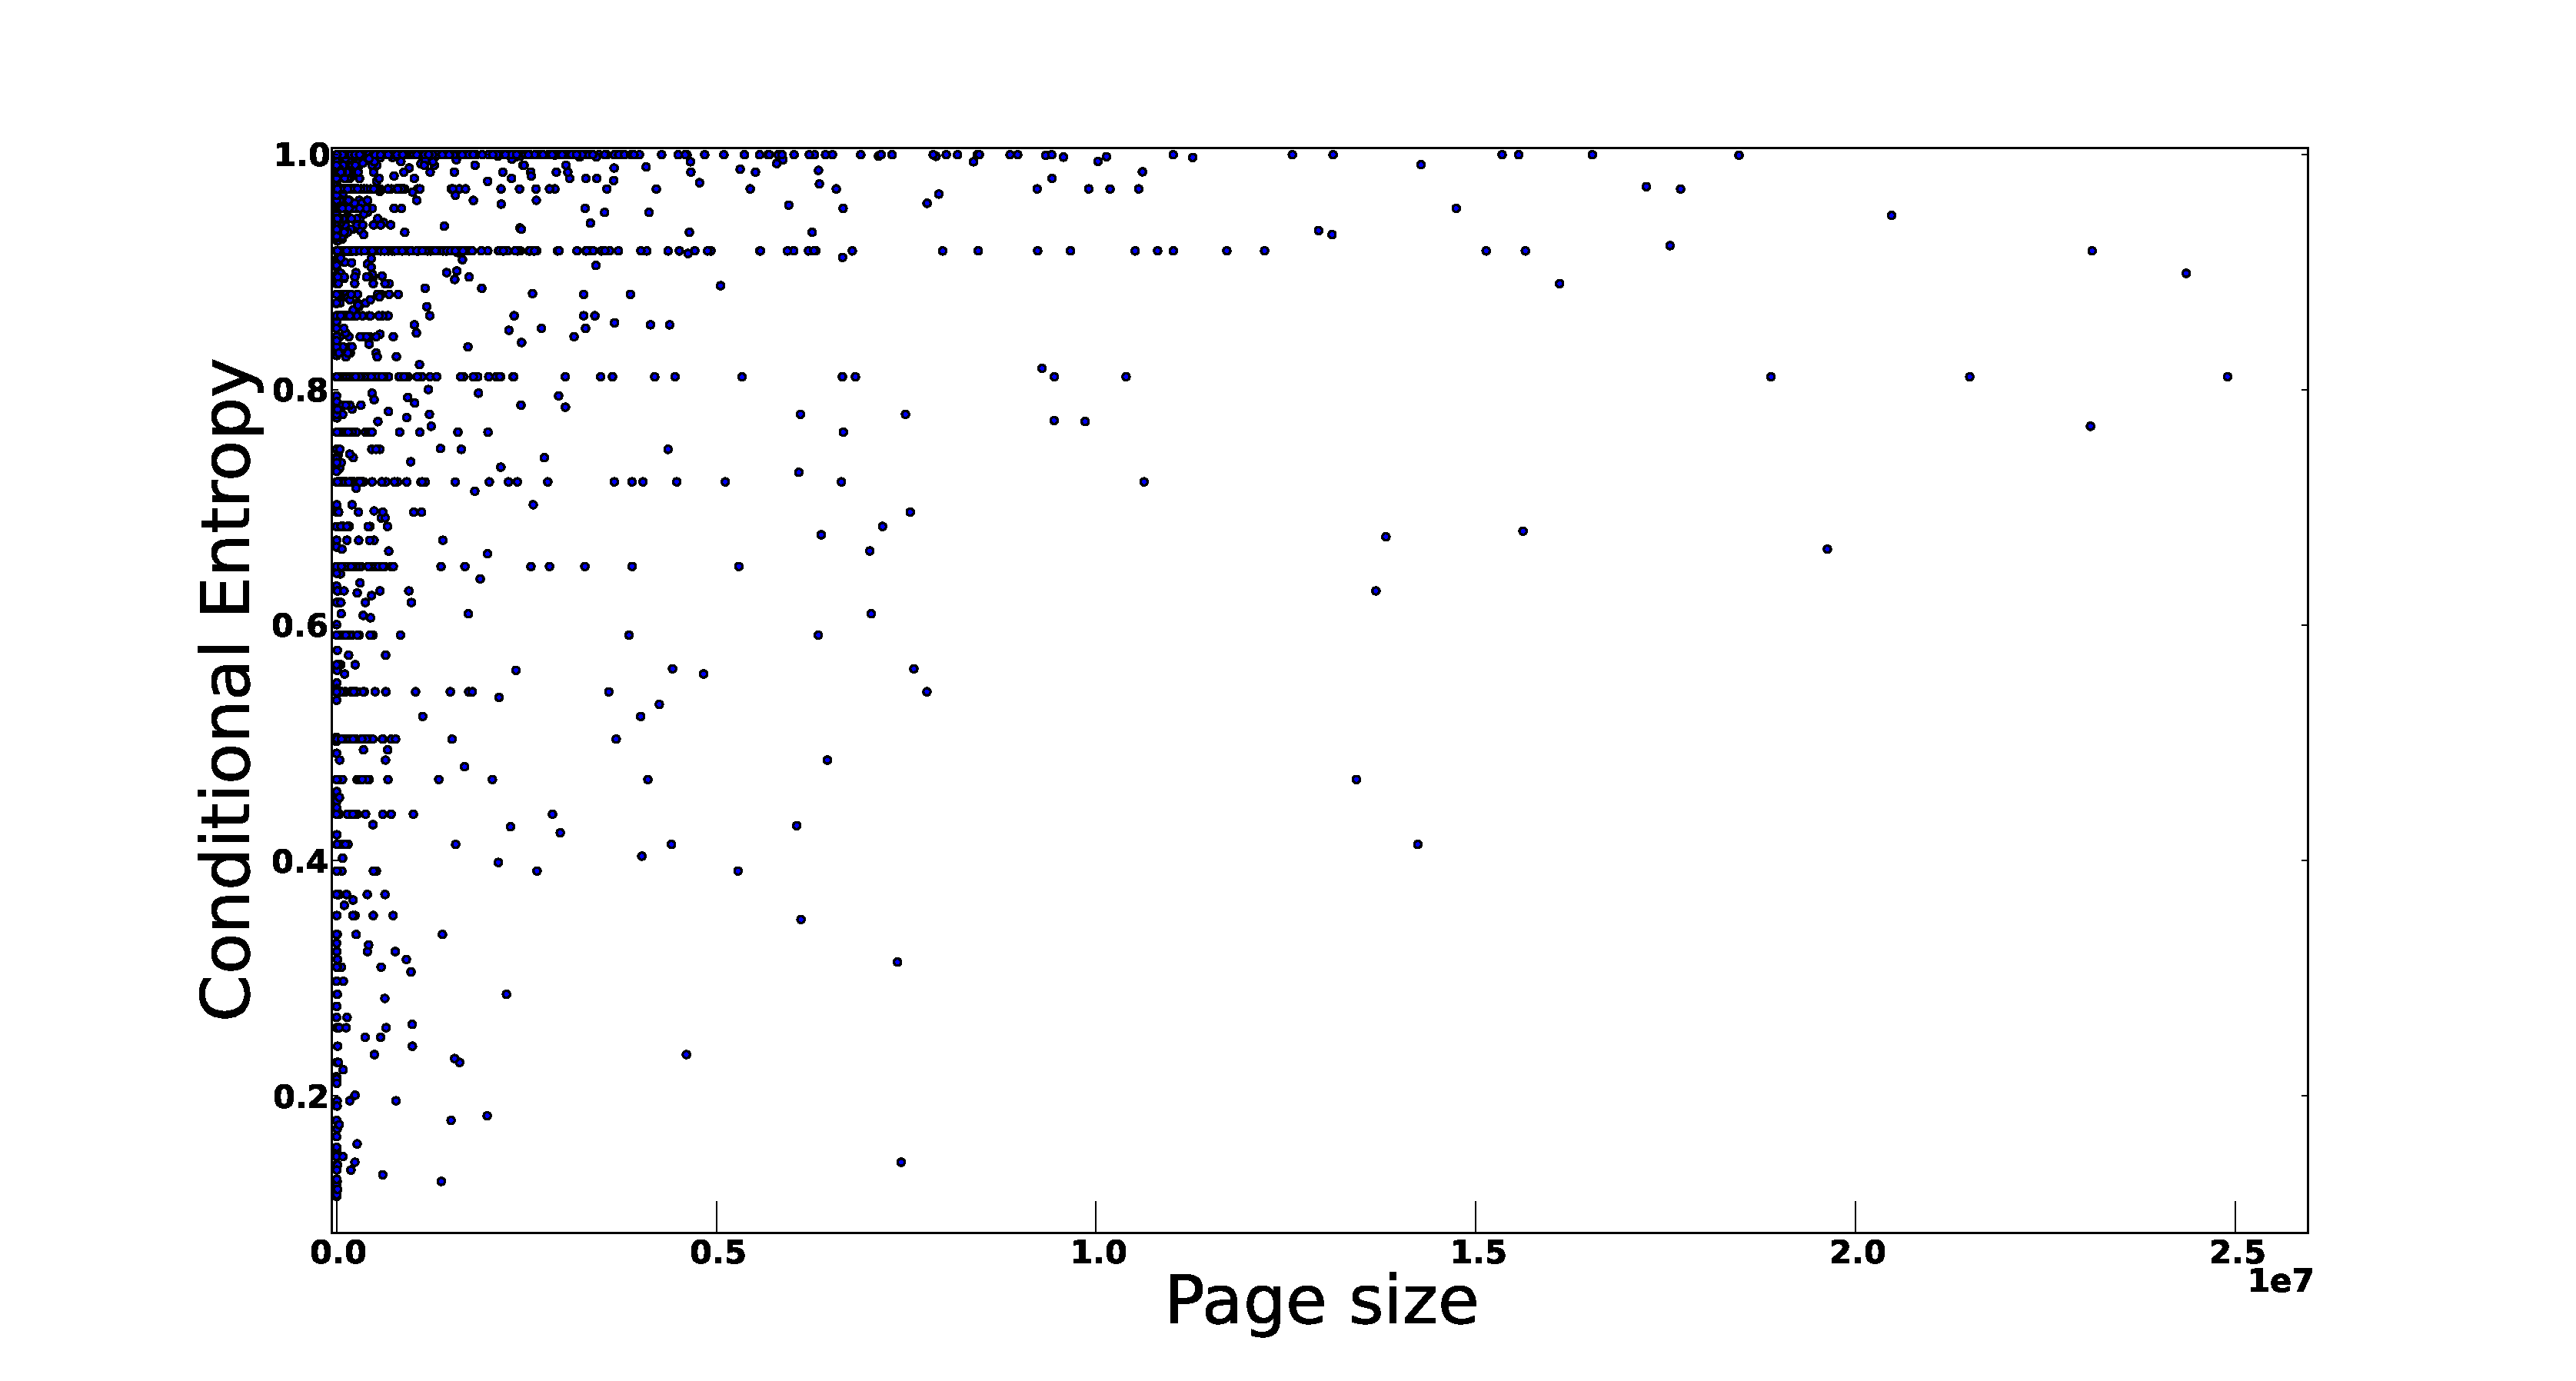
\includegraphics[width=45mm, height=35mm]{data/plots/new/CEvsPageSize.eps}}
\subfloat[Fig:][]{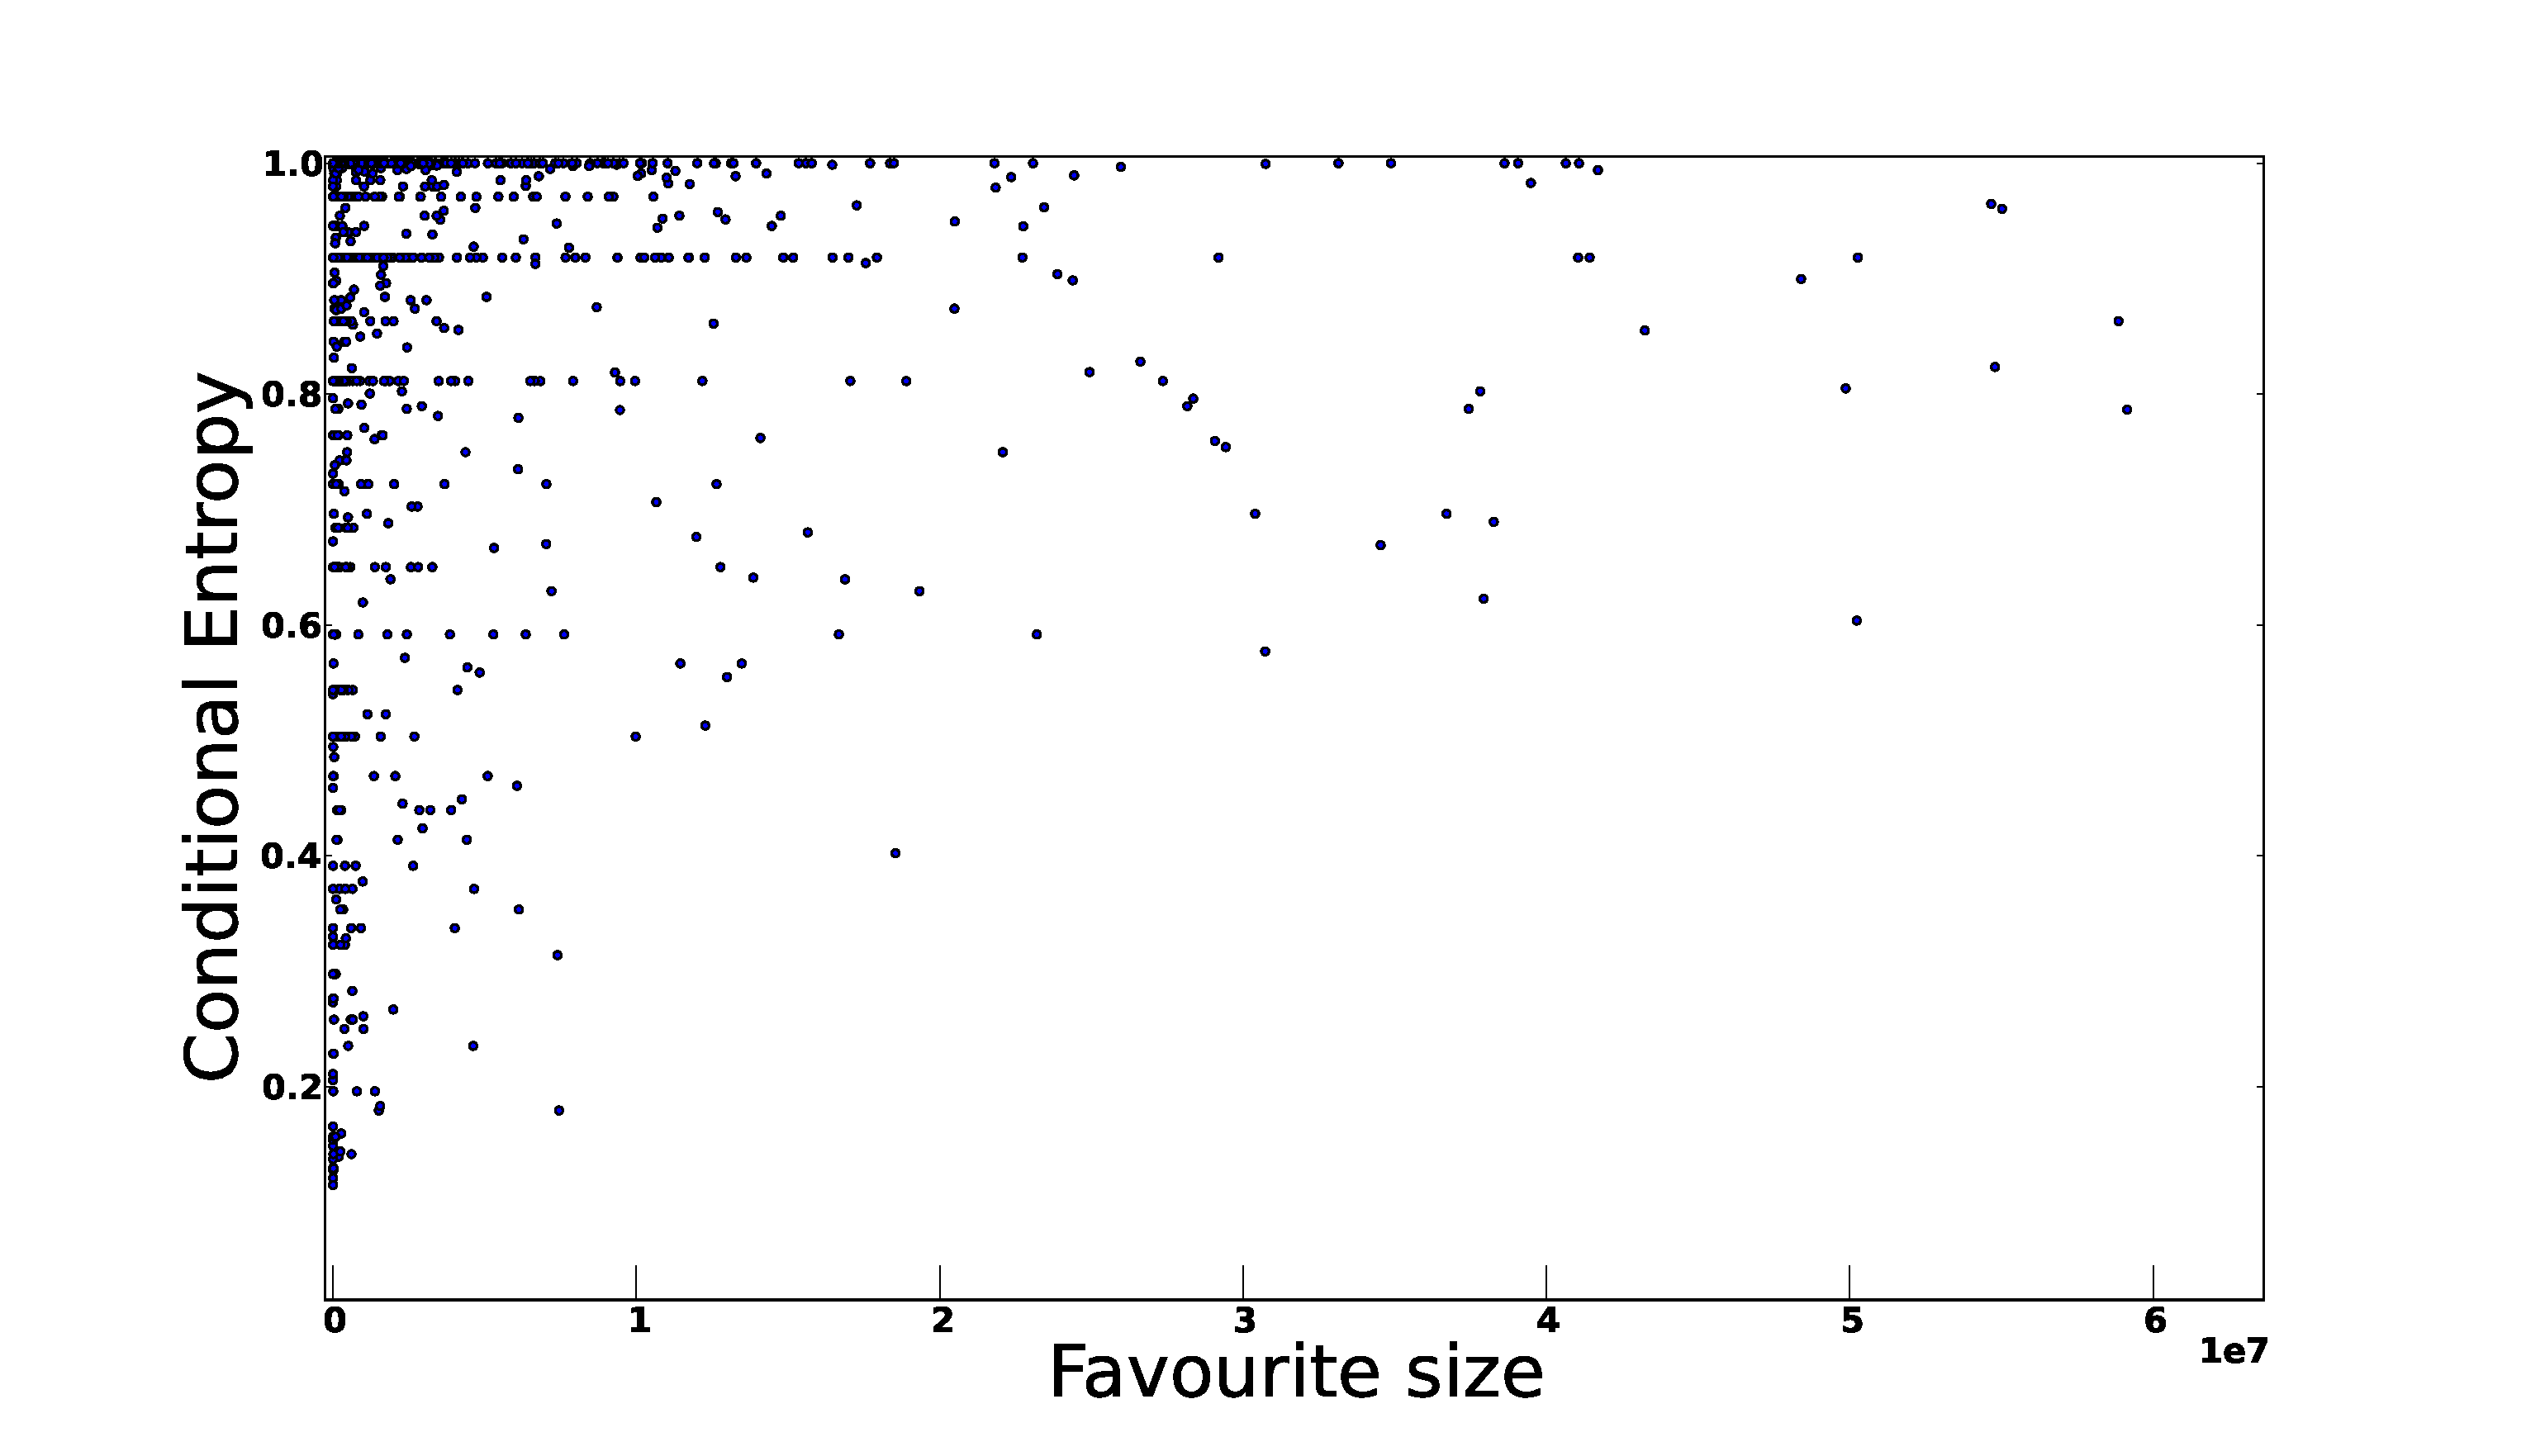
\includegraphics[width=45mm, height=35mm]{data/plots/new/CEvsFavSize.eps}} \\
\subfloat[Fig:][]{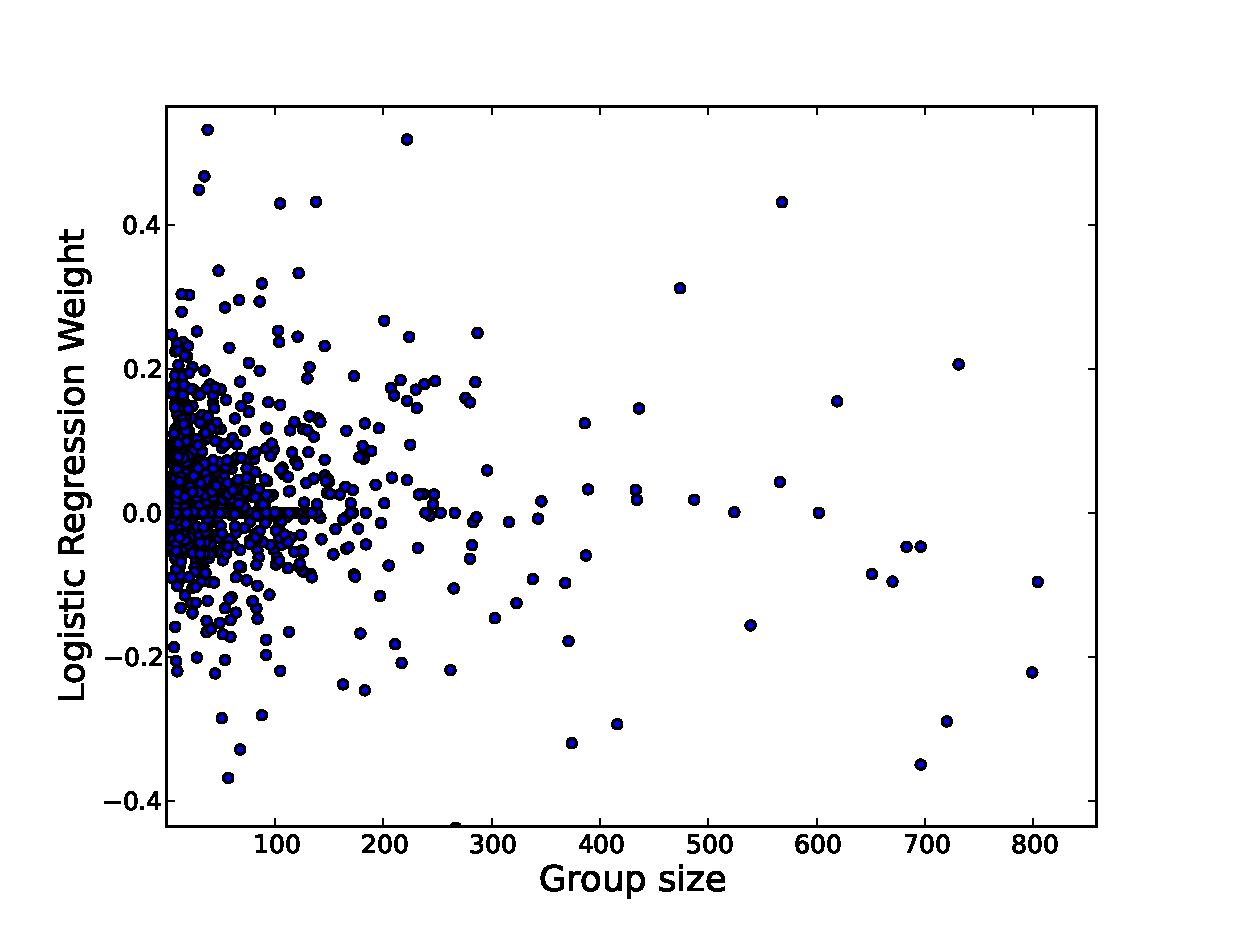
\includegraphics[width=45mm, height=35mm]{data/plots/new/LRweightvsGroupSize.eps}}
\subfloat[Fig:][]{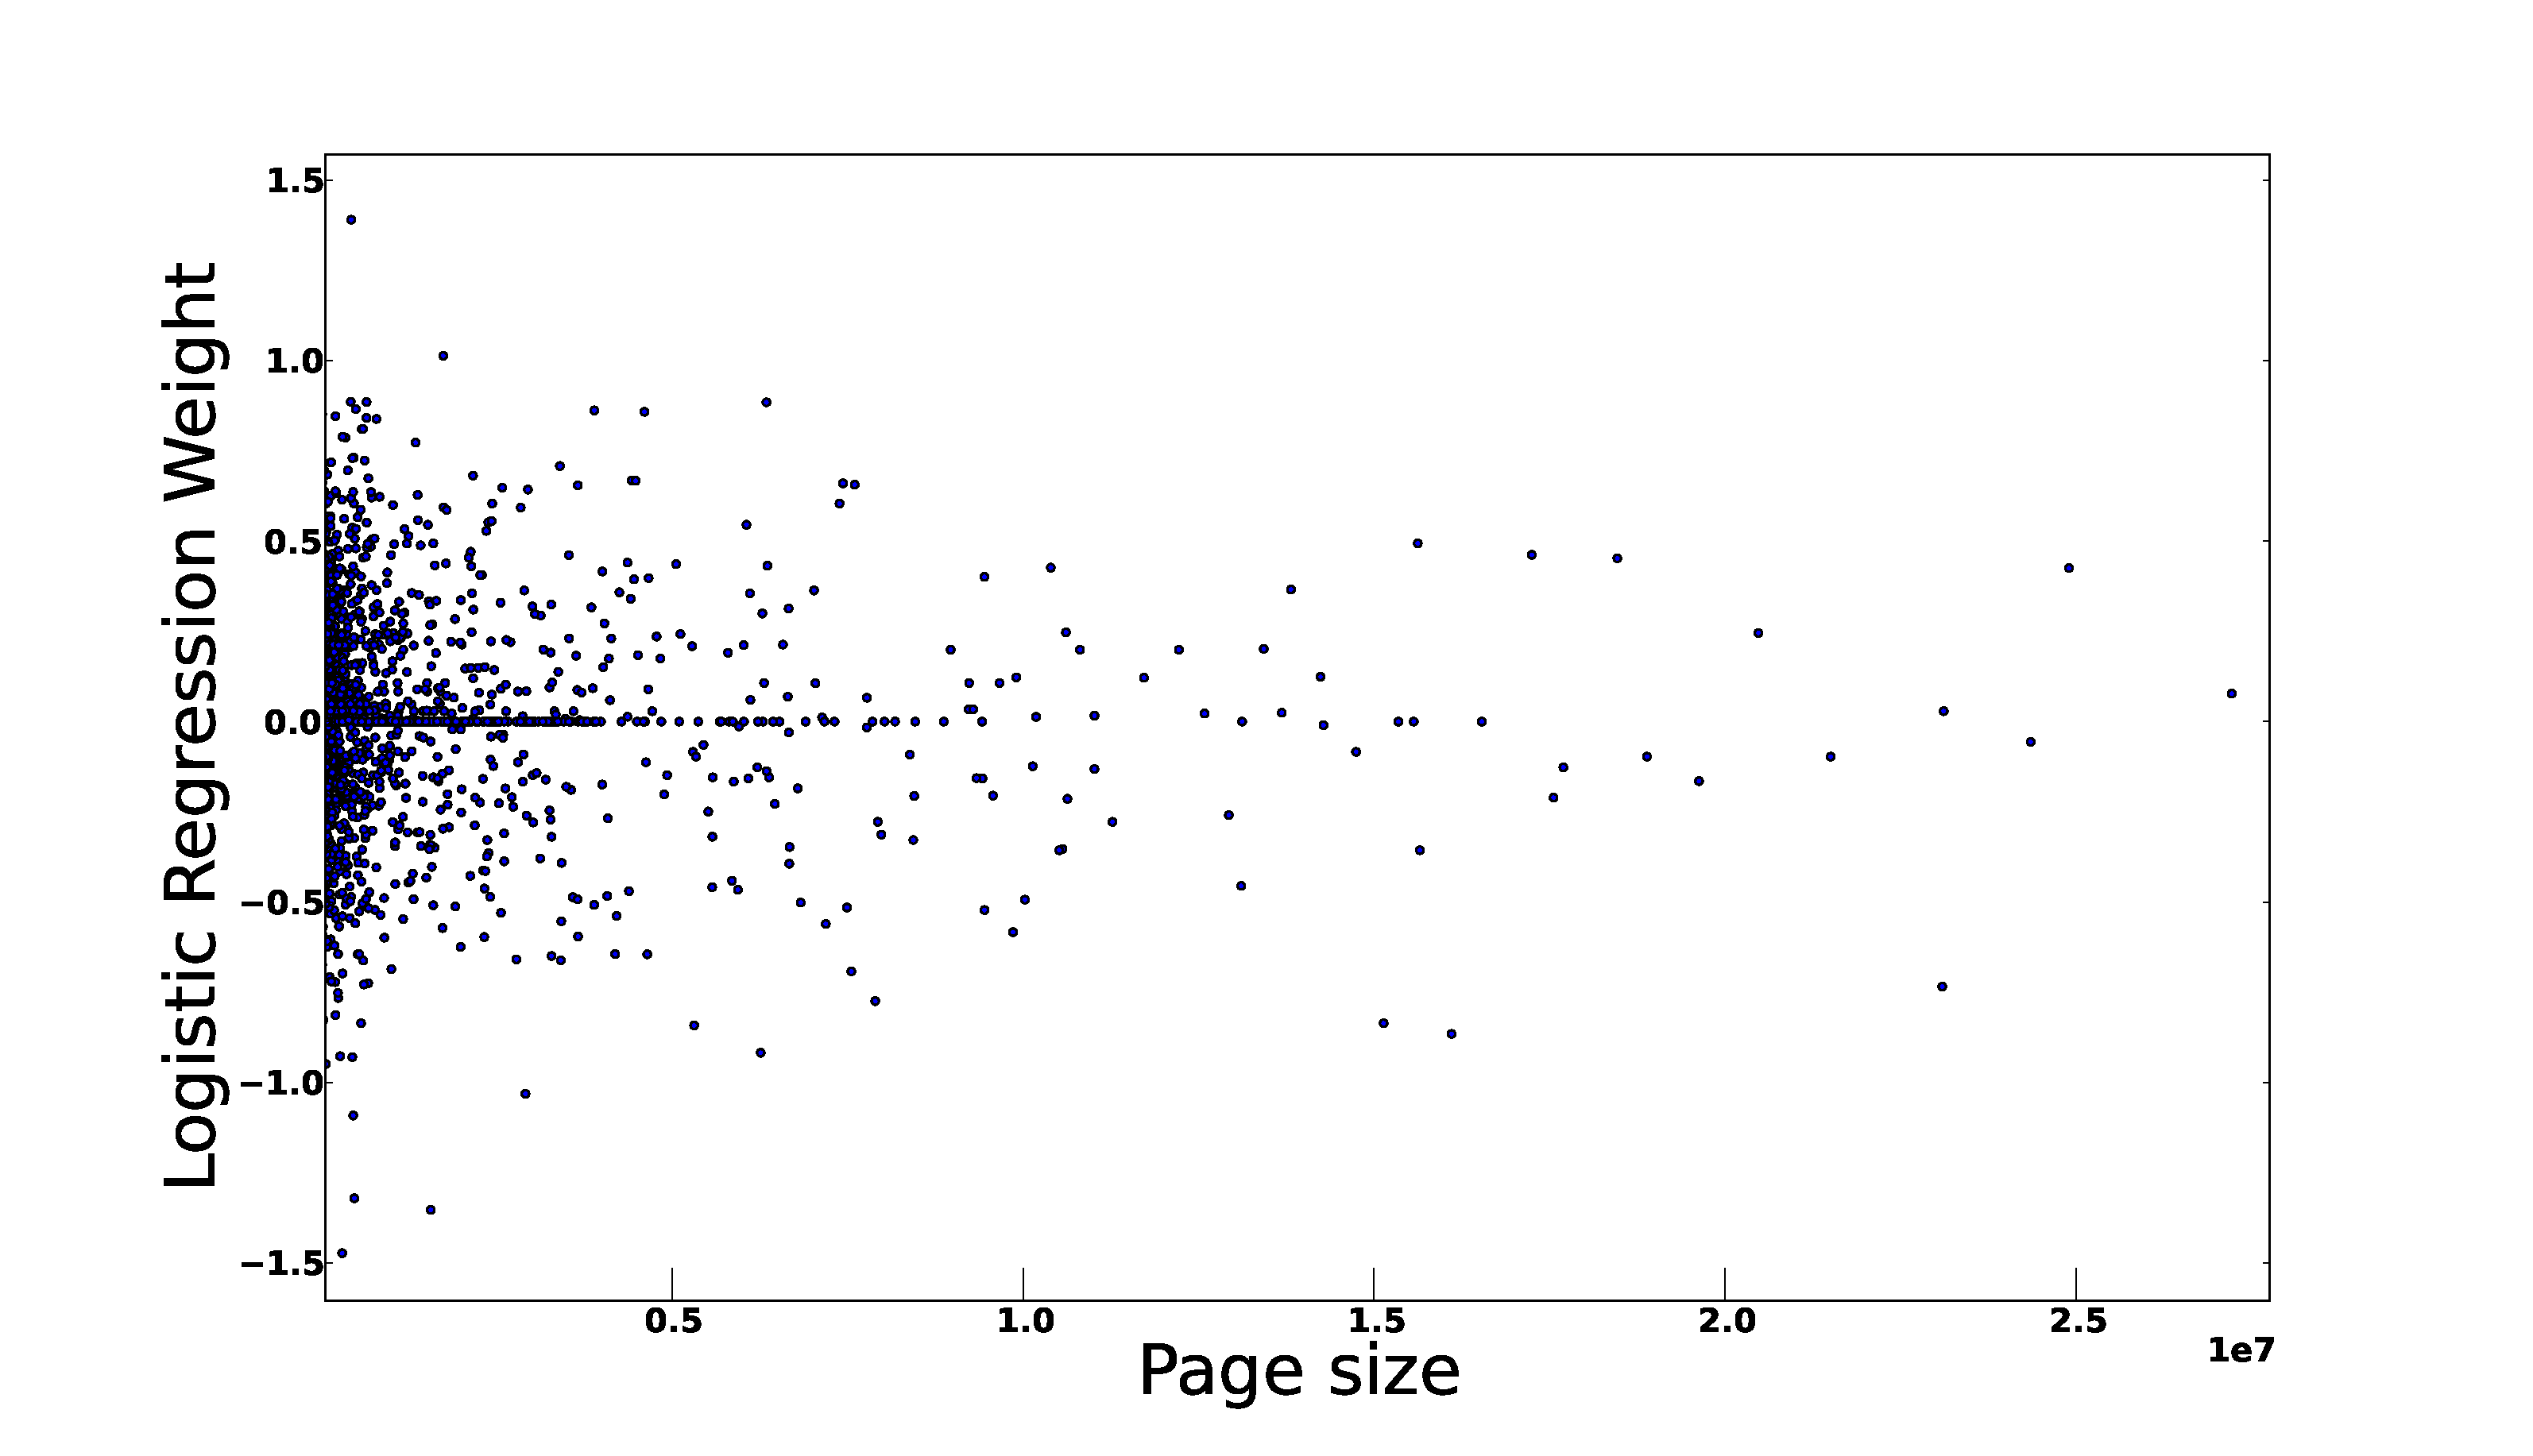
\includegraphics[width=45mm, height=35mm]{data/plots/new/LRweightvsPageSize.eps}}
\subfloat[Fig:][]{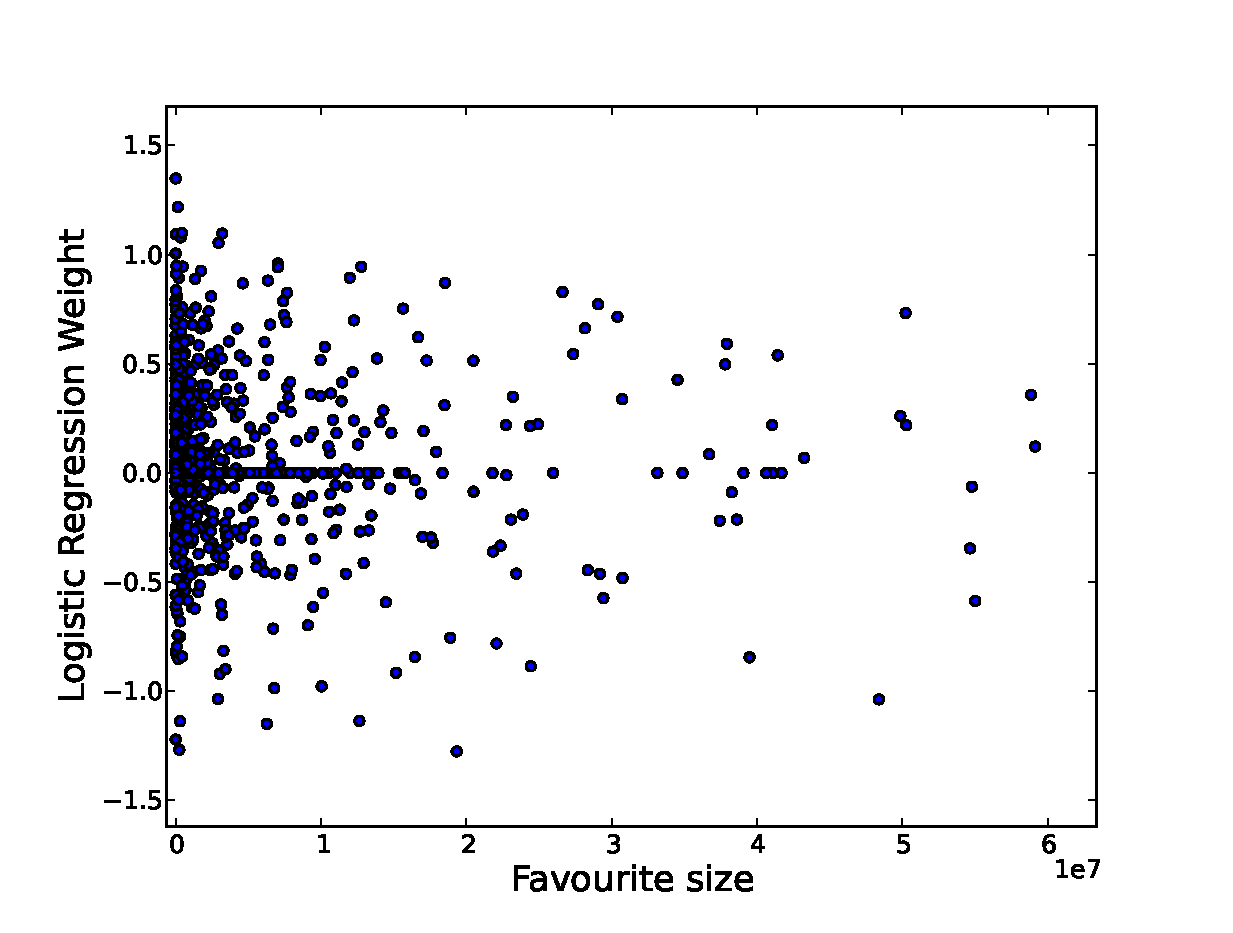
\includegraphics[width=45mm, height=35mm]{data/plots/new/LRweightvsFavSize.eps}} \\
\end{tabular}
\end{tabular}
\caption {Conditional entropy vs size (a-c); logistic regression feature weights vs size (d-f) }
\label{Fig3}
\end{figure*}
%%%%%%%%%%%%%%%%%%%%%%%%%%%%%%%%%%%%%%%%%%%%%%%%%%%%%%%%%%%%%%%%%%%%%%%%%%%

%%%%%%%%%%%%%%%%%%%%%%%%%%%%%%%%%%%%%%%%%%%%%%%%%%%%%%%%%%%%%%%%%%%%%%%%%%%
\begin{figure*}[tbp!]
\centering
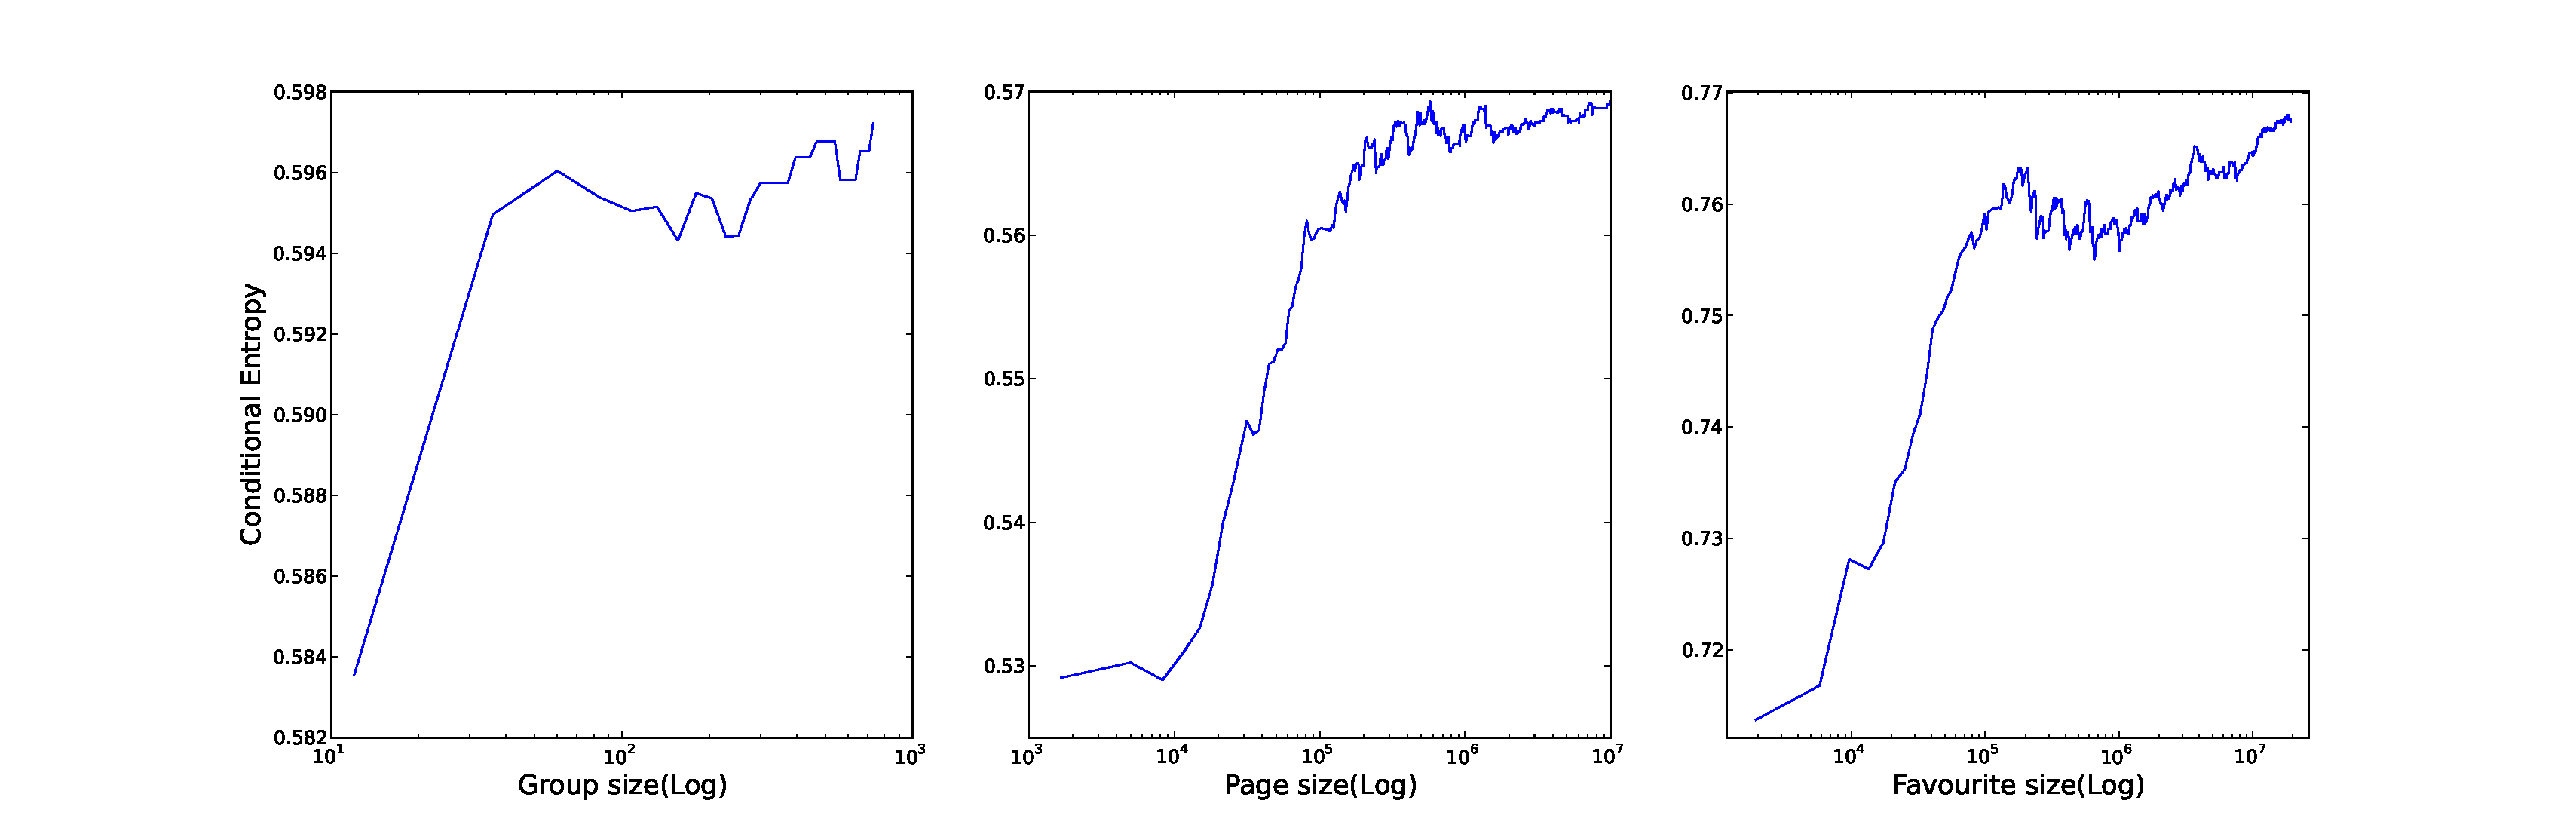
\includegraphics[scale=0.28]{data/plots/cumulativeEntropy/cumulative.eps}
\caption{Average conditional entropy of top 10\% groups, pages and favourites features cumulative over the size }
\label{Fig4}
\end{figure*}
%%%%%%%%%%%%%%%%%%%%%%%%%%%%%%%%%%%%%%%%%%%%%%%%%%%%%%%%%%%%%%%%%%%%%%%%%%%

%%%%%%%%%%%%%%%%%%%%%%%%%%%%%%%%%%%%%%%%%%%%%%%%%%%%%%%%%%%%%%%%%%%%%%%%%%%
\begin{figure*}[tbp!]
\centering
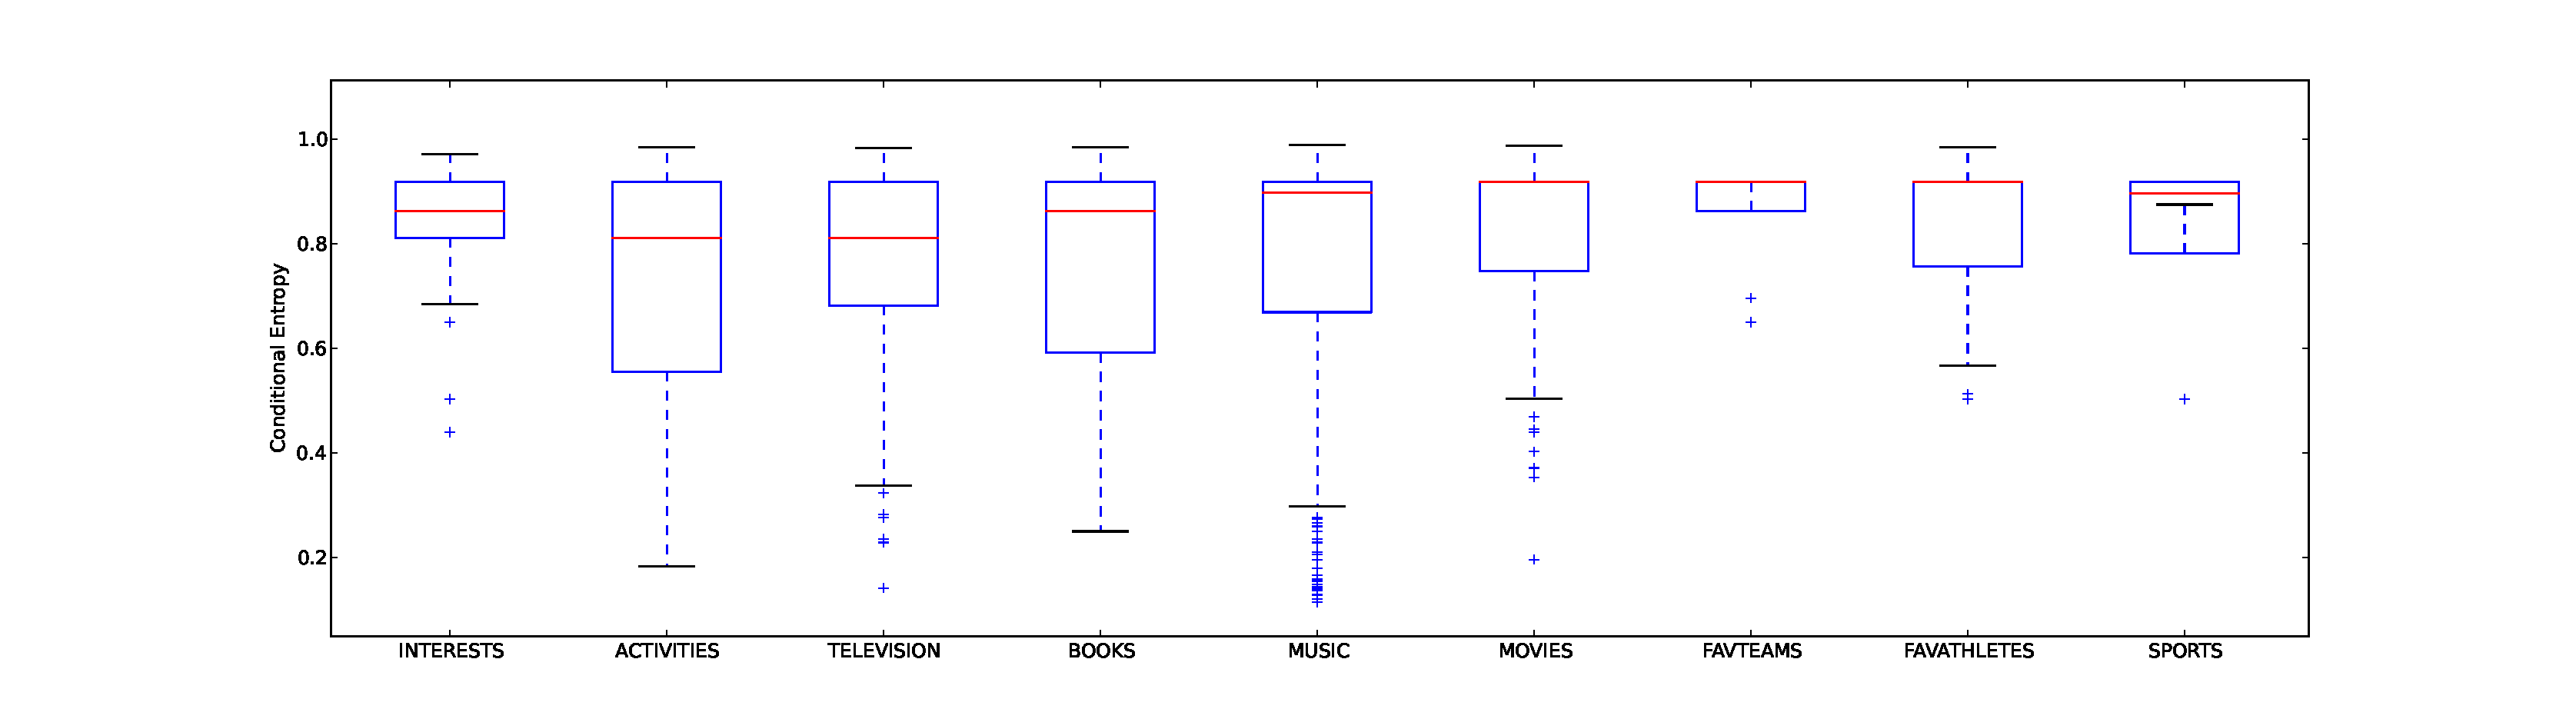
\includegraphics[width=180mm, height=40mm]{data/plots/boxPlots/CEvsFavTypes.eps}
\caption{Conditional entropy for top 1000 favourites breakdown by categories}
\label{Fig5}
\end{figure*}
%%%%%%%%%%%%%%%%%%%%%%%%%%%%%%%%%%%%%%%%%%%%%%%%%%%%%%%%%%%%%%%%%%%%%%%%%%%


\section{Related Work}


%There has been many recent work on inferring user preferences on information 
 
This work relates to many others in inferring user preferences on social and information networks. 
We structure the discussion into two parts: the first is concerned with the nature of user traits, interactions and diffusion, the second is concerned with relating these user traits and interactions to  user preferences, interests and the strength of social ties.

%To structure the discussion, we categorize the observables into three types:
%There are three main types of observables in such networks 
%(1) {\em User profile} including friendship information, they change at a much slower rate than information propagation in the network; (2) a dynamic stream of {\em interactions}, between users or between a user and a digital object; (3) a global and networked view of interactions, i.e. {\em diffusion} cascades. There are two types of hidden information that are common targets of inference and prediction: (a) User {\em preference} and interest, sometimes expressed as positive and negative (e.g. likes, voting up or down) action; (b) the inherent strength of {\em social ties}. 
%While the main objective of our study is to correlate 
%interactions and profile to user preference, 

The first group studies the nature of user profile, interactions, and diffusion.
Profile information and demographics is correlated with user behavior
patterns. \cite{Chang2010ethnicity} showed that the tendency to
initiate a Facebook friendship differs quite widely across ethnical
groups, while \cite{backstrom2011center} have additionally showed that female and male users have opposite tendencies for dispersing attention for within-gender and across-gender communication.
Two particular measurement studies on Facebook attention~\cite{wilson2009user,backstrom2011center} have inspired our work.  Although the average number of friends for a Facebook user is close to the human psychological limit, known as the Dunbar number~\cite{hill2003social}, the findings concur that a user's attention (i.e., interactions) are divided among a much smaller subset of Facebook friends. \cite{backstrom2011center} studied two types of attention: communication interaction and viewing attention (e.g. looking at profiles or photos). Users' communication attention is focused on small numbers of friends, but viewing attention is dispersed across all friends.
This finding supports our approach of looking at many types of user interactions across all of a user's contact network, as a user's interest is driven by where he or she focuses attention on.

The mechanisms of diffusion invites interesting mathematical and empirical investigations. %of diffusion has generated many interesting observations. 
The Galton�Watson epidemics model suits the basic setup of social
message diffusion, and can explain real-world information cascade such as
email chain-letters when adjusted with selection
bias~\cite{Golub2010selectionbiase}. For social diffusions in a
one-to-many setting, however, the epidemics model has been less
accurate. \cite{ver2011stops} found that online message cascades (on
Digg social reader) are often smaller than prescribed by the epidemics
model, seemingly due to the diminishing returns of repeated
exposure. \cite{Romero2011hashtag}, in an independent study, confirmed
the effect of diminishing returns with Twitter hashtag cascades, and
further found that cascade dynamics differ across broad topic
categories such as politics, culture, or sports. Our observations on a number of Facebook interactions agrees with the effect of diminishing returns.

The nature of social diffusion seem to be not only democratic~\cite{asur2011trends,Bakshy2011everyone}, but also broadening for users~\cite{Bakshy2012chamber}. While influential users are important for cascade generation~\cite{Bakshy2011everyone}, large active groups of users are needed to contribute for the cascade to sustain~\cite{asur2011trends}. Moreover, word-of-mouth diffusion can only be harnessed reliably by targeting large numbers of potential influencers, confirmed by observations on Twitter~\cite{Bakshy2011everyone} and online ads~\cite{influence}. In a study facilitated by A/B testing on Facebook links, \cite{Bakshy2012chamber} found that while people are more likely to share the information they were exposed to by their strong ties than by their weak ties, the bulk of information we consume and share comes from people with different perspectives (weak ties). Our Facebook App is intended to bridge this gap between insights from these observations and predicting user actions.

The second group of related work tries to correlate from user interactions to preferences and tie strength. 
~\cite{saez2011high} found that incoming and outgoing actives are
highly correlated on broadcast platforms such as Facebook and Twitter,
and such correlation does not hold in one-to-one mode of communication
such as email. Multiple studies have found that online interactions
tend to correlate more with interests than with user profile. \cite{singla2008yes} found that user who frequently interact (via MSN chat) tend to share (web search) interests. 
\cite{Anderson2012} concluded that the level of user activities correlate with the positive ratings that they give each other, and it is less about what they say (content of posts) but more about who they interacted with. Such findings echo those by ~\cite{brandtzag2011facebook}
that real-world interactions further strengthens friendship on Facebook, while virtual interactions reveal interests. Furthermore, ratings of real-world friendship strength and trust~\cite{gilbert2009predicting} seems to be more predictable from the intimacy, intensity, and duration of interactions, than from social distance and structural information. 
In terms of making the interaction-to-preference operational, \cite{nori2011exploiting} examines the predictability of user actions on Twitter from actions in both Twitter and Del.icio.us. The study uses both linear regression and an bipartite graph model that outperformed state-of-the-art models. ~\cite{gomes2011social} derived rules for Facebook interactions using a psychology-inspired formal symbolic language. 
These work are most closely related to ours, yet none has examined such a diverse set of user actions in the same context: one-on-one interactions (e.g. commenting), broadcast (e.g. posting, sharing), and co-preference (e.g. likes). 
%From data mining these rules, ranking them on confidence and support, the study found users are more likely to `like' another user's post or comment than to actively comment on it, and that the action of a `like' or `comment' by one user does not affect the involvement of other users in social interactions.

In summary, our study is motivated by overall utility of weak ties, diverse, and very specific interactions. To the best of our knowledge, this is the first work that look at all of various combinations of interactions and user traits outlined in our Methodology.  Our preliminary findings confirm many of the observations made in the literature while shedding new light on some of these effects (and new causes of these effects) for a rich set of Facebook user and interaction data.


\section{Conclusions}

\input conclusion

\bibliography{bibliography}
\bibliographystyle{abbrv}

\end{document}

